% Options for packages loaded elsewhere
\PassOptionsToPackage{unicode}{hyperref}
\PassOptionsToPackage{hyphens}{url}
%
\documentclass[
  twocolumn,
  10pt,
  a4paper]{article}
\usepackage{amsmath,amssymb}
\usepackage{iftex}
\ifPDFTeX
  \usepackage[T1]{fontenc}
  \usepackage[utf8]{inputenc}
  \usepackage{textcomp} % provide euro and other symbols
\else % if luatex or xetex
  \usepackage{unicode-math} % this also loads fontspec
  \defaultfontfeatures{Scale=MatchLowercase}
  \defaultfontfeatures[\rmfamily]{Ligatures=TeX,Scale=1}
\fi
\usepackage{lmodern}
\ifPDFTeX\else
  % xetex/luatex font selection
  \setmainfont[]{DejaVu Serif}
  \setmonofont[]{DejaVu Sans Mono}
\fi
% Use upquote if available, for straight quotes in verbatim environments
\IfFileExists{upquote.sty}{\usepackage{upquote}}{}
\IfFileExists{microtype.sty}{% use microtype if available
  \usepackage[]{microtype}
  \UseMicrotypeSet[protrusion]{basicmath} % disable protrusion for tt fonts
}{}
\makeatletter
\@ifundefined{KOMAClassName}{% if non-KOMA class
  \IfFileExists{parskip.sty}{%
    \usepackage{parskip}
  }{% else
    \setlength{\parindent}{0pt}
    \setlength{\parskip}{6pt plus 2pt minus 1pt}}
}{% if KOMA class
  \KOMAoptions{parskip=half}}
\makeatother
\usepackage{xcolor}
\usepackage{color}
\usepackage{fancyvrb}
\newcommand{\VerbBar}{|}
\newcommand{\VERB}{\Verb[commandchars=\\\{\}]}
\DefineVerbatimEnvironment{Highlighting}{Verbatim}{commandchars=\\\{\}}
% Add ',fontsize=\small' for more characters per line
\newenvironment{Shaded}{}{}
\newcommand{\AlertTok}[1]{\textcolor[rgb]{1.00,0.00,0.00}{\textbf{#1}}}
\newcommand{\AnnotationTok}[1]{\textcolor[rgb]{0.38,0.63,0.69}{\textbf{\textit{#1}}}}
\newcommand{\AttributeTok}[1]{\textcolor[rgb]{0.49,0.56,0.16}{#1}}
\newcommand{\BaseNTok}[1]{\textcolor[rgb]{0.25,0.63,0.44}{#1}}
\newcommand{\BuiltInTok}[1]{\textcolor[rgb]{0.00,0.50,0.00}{#1}}
\newcommand{\CharTok}[1]{\textcolor[rgb]{0.25,0.44,0.63}{#1}}
\newcommand{\CommentTok}[1]{\textcolor[rgb]{0.38,0.63,0.69}{\textit{#1}}}
\newcommand{\CommentVarTok}[1]{\textcolor[rgb]{0.38,0.63,0.69}{\textbf{\textit{#1}}}}
\newcommand{\ConstantTok}[1]{\textcolor[rgb]{0.53,0.00,0.00}{#1}}
\newcommand{\ControlFlowTok}[1]{\textcolor[rgb]{0.00,0.44,0.13}{\textbf{#1}}}
\newcommand{\DataTypeTok}[1]{\textcolor[rgb]{0.56,0.13,0.00}{#1}}
\newcommand{\DecValTok}[1]{\textcolor[rgb]{0.25,0.63,0.44}{#1}}
\newcommand{\DocumentationTok}[1]{\textcolor[rgb]{0.73,0.13,0.13}{\textit{#1}}}
\newcommand{\ErrorTok}[1]{\textcolor[rgb]{1.00,0.00,0.00}{\textbf{#1}}}
\newcommand{\ExtensionTok}[1]{#1}
\newcommand{\FloatTok}[1]{\textcolor[rgb]{0.25,0.63,0.44}{#1}}
\newcommand{\FunctionTok}[1]{\textcolor[rgb]{0.02,0.16,0.49}{#1}}
\newcommand{\ImportTok}[1]{\textcolor[rgb]{0.00,0.50,0.00}{\textbf{#1}}}
\newcommand{\InformationTok}[1]{\textcolor[rgb]{0.38,0.63,0.69}{\textbf{\textit{#1}}}}
\newcommand{\KeywordTok}[1]{\textcolor[rgb]{0.00,0.44,0.13}{\textbf{#1}}}
\newcommand{\NormalTok}[1]{#1}
\newcommand{\OperatorTok}[1]{\textcolor[rgb]{0.40,0.40,0.40}{#1}}
\newcommand{\OtherTok}[1]{\textcolor[rgb]{0.00,0.44,0.13}{#1}}
\newcommand{\PreprocessorTok}[1]{\textcolor[rgb]{0.74,0.48,0.00}{#1}}
\newcommand{\RegionMarkerTok}[1]{#1}
\newcommand{\SpecialCharTok}[1]{\textcolor[rgb]{0.25,0.44,0.63}{#1}}
\newcommand{\SpecialStringTok}[1]{\textcolor[rgb]{0.73,0.40,0.53}{#1}}
\newcommand{\StringTok}[1]{\textcolor[rgb]{0.25,0.44,0.63}{#1}}
\newcommand{\VariableTok}[1]{\textcolor[rgb]{0.10,0.09,0.49}{#1}}
\newcommand{\VerbatimStringTok}[1]{\textcolor[rgb]{0.25,0.44,0.63}{#1}}
\newcommand{\WarningTok}[1]{\textcolor[rgb]{0.38,0.63,0.69}{\textbf{\textit{#1}}}}
\usepackage{longtable,booktabs,array}
\usepackage{calc} % for calculating minipage widths
% Correct order of tables after \paragraph or \subparagraph
\usepackage{etoolbox}
\makeatletter
\patchcmd\longtable{\par}{\if@noskipsec\mbox{}\fi\par}{}{}
\makeatother
% Allow footnotes in longtable head/foot
\IfFileExists{footnotehyper.sty}{\usepackage{footnotehyper}}{\usepackage{footnote}}
\makesavenoteenv{longtable}
\usepackage{graphicx}
\makeatletter
\def\maxwidth{\ifdim\Gin@nat@width>\linewidth\linewidth\else\Gin@nat@width\fi}
\def\maxheight{\ifdim\Gin@nat@height>\textheight\textheight\else\Gin@nat@height\fi}
\makeatother
% Scale images if necessary, so that they will not overflow the page
% margins by default, and it is still possible to overwrite the defaults
% using explicit options in \includegraphics[width, height, ...]{}
\setkeys{Gin}{width=\maxwidth,height=\maxheight,keepaspectratio}
% Set default figure placement to htbp
\makeatletter
\def\fps@figure{htbp}
\makeatother
\setlength{\emergencystretch}{3em} % prevent overfull lines
\providecommand{\tightlist}{%
  \setlength{\itemsep}{0pt}\setlength{\parskip}{0pt}}
\setcounter{secnumdepth}{-\maxdimen} % remove section numbering
\ifLuaTeX
\usepackage[bidi=basic]{babel}
\else
\usepackage[bidi=default]{babel}
\fi
\babelprovide[main,import]{english}
\ifPDFTeX
\else
\babelfont{rm}[]{DejaVu Serif}
\fi
% get rid of language-specific shorthands (see #6817):
\let\LanguageShortHands\languageshorthands
\def\languageshorthands#1{}
% TruthSpace paper preamble -- IEEE-inspired twocolumn layout
% Loaded via pandoc --include-in-header to keep raw LaTeX intact.

\usepackage{float}
\usepackage{array}
\usepackage{etoolbox}

% dblfloatfix improves placement of \begin{figure*} (two-column-
% spanning floats).  Without it, LaTeX 2e tends to defer wide floats
% to the end of a chapter or onto float-only pages.  With dblfloatfix
% wide floats can land at the bottom of a column and flow more
% naturally with the text that references them.
\usepackage{dblfloatfix}

% seqsplit lets us break long monospace identifiers (file paths,
% function names with underscores) anywhere, which prevents the
% otherwise-unhyphenable \texttt{...} runs from overflowing a
% narrow column.  Used by the post-process step in build_paper.sh
% to wrap any long inline \texttt content.
\usepackage{seqsplit}

% Caption styling.  We suppress LaTeX's auto "Figure N." prefix because
% the markdown captions already include their own chapter-prefixed labels
% ("Figure 3.1:", "Figure B.6:", etc.).  Without this, captions would
% render as "Figure 5. Figure 3.1: ..." (doubled).
\usepackage[font=small,labelformat=empty,labelsep=none]{caption}

% Keep figures inside the chapter (\section in this article-class
% paper) they belong to so floats don't migrate across major
% boundaries, but allow them to flow within a chapter (subsection
% boundaries don't introduce \FloatBarrier).  Without this, large
% wide-figure floats migrate to the wrong place; with [section] they
% used to get isolated on their own pages.  We balance this by adding
% a manual \FloatBarrier before each \chapter-equivalent (the level-1
% section) inside the post-process.
\usepackage{placeins}

% Tighter column gutter and float spacing
\setlength{\columnsep}{18pt}
\setlength{\textfloatsep}{8pt}
\setlength{\intextsep}{8pt}

% Float-placement fractions tuned for wide figures (figure*) so they
% can land at the top or bottom of regular text pages instead of
% being banished to float-only pages.  LaTeX defaults are very
% conservative (topfraction=0.7, dbltopfraction=0.7,
% floatpagefraction=0.5) which routinely rejects a 4-inch-tall
% figure on a 9-inch text column.  These looser values keep wide
% figures with their text reference.
\renewcommand{\topfraction}{0.92}
\renewcommand{\bottomfraction}{0.85}
\renewcommand{\dbltopfraction}{0.92}
\renewcommand{\textfraction}{0.08}
\renewcommand{\floatpagefraction}{0.85}
\renewcommand{\dblfloatpagefraction}{0.85}

% Default every \includegraphics{} to \linewidth (graphicx is already
% loaded by pandoc earlier in the preamble).  \linewidth equals
% \columnwidth in single-column blocks and \textwidth in figure*
% (two-column-spanning) floats, so multi-panel figures promoted to
% figure* by the build_paper.sh post-process automatically fill the
% page width.
\setkeys{Gin}{width=\linewidth,keepaspectratio}

% Code blocks at column width.  Pandoc defines the Highlighting
% environment via \DefineVerbatimEnvironment with the base fancyvrb
% package, but fancyvrb does not provide line-breaking options.
% Load fvextra (a superset of fancyvrb) which adds breaklines/
% breakanywhere, and use \RecustomVerbatimEnvironment to override
% the pandoc definition with our breaking-enabled options.
\usepackage{fvextra}
\RecustomVerbatimEnvironment{Highlighting}{Verbatim}{%
  commandchars=\\\{\},%
  breaklines=true,%
  breakanywhere=true,%
  fontsize=\scriptsize}
% Also apply to plain verbatim code blocks (pandoc's `verbatim`
% environment), which lack syntax highlighting.
\fvset{breaklines=true,breakanywhere=true,fontsize=\scriptsize}

% Redirect plain LaTeX `verbatim` (used by pandoc for code blocks
% without a language tag) to fancyvrb's `Verbatim`, so that the
% breaklines/breakanywhere settings above apply to *every* code
% block in the paper.  Without this, an un-labelled triple-backtick
% block (e.g. the pseudocode skeleton in 1.4) typesets as a plain
% verbatim and overflows the column at long lines.
\renewenvironment{verbatim}
  {\VerbatimEnvironment\begin{Verbatim}}
  {\end{Verbatim}}

% Pandoc emits a longtable environment for every markdown table.
% longtable doesn't work in twocolumn mode, so build_paper.sh
% post-processes each one into a centred footnotesize tabularx of
% column width.  See the post-process step in build_paper.sh for the
% full token rewriting (the comment patterns there avoid putting
% literal longtable begin/end tokens in this preamble).
%
% A wide table that should span both columns can be wrapped in raw
% LaTeX table-star markup in the markdown source: tabularx's
% \linewidth then expands to \textwidth (full two-column width).
%
% endhead / endfirsthead / endfoot / endlastfoot get \let-relaxed so
% any surviving longtable-syntax commands are no-ops.
\usepackage{tabularx}
\newcolumntype{Y}{>{\raggedright\arraybackslash}X}
\newenvironment{tsxtable}{\begin{center}\footnotesize}{\end{center}}
\let\endhead\relax
\let\endfirsthead\relax
\let\endfoot\relax
\let\endlastfoot\relax

% Figure dividers.  A simple centred thin rule inserted at the top
% and bottom of every floated figure so readers can tell where the
% figure starts and ends when it lands in the middle of a page
% (between paragraphs of body text).  At a page edge the rule sits
% against the margin and the page boundary itself serves as a
% divider, which is harmless.  The rule has the same width and
% weight as the chapter-section separators that pandoc emits for
% markdown horizontal rules (---), so figure dividers blend
% visually with section breaks rather than introducing a second
% divider style.
\newcommand{\figdivider}{%
  \par\addvspace{4pt}%
  {\centering\rule{0.5\linewidth}{0.5pt}\par}%
  \addvspace{2pt}%
}
% Hook the divider into every figure / figure* float so the
% ornament travels with the float to wherever LaTeX places it.
\AtBeginEnvironment{figure}{\figdivider}
\AtEndEnvironment{figure}{\figdivider}
\AtBeginEnvironment{figure*}{\figdivider}
\AtEndEnvironment{figure*}{\figdivider}
\ifLuaTeX
  \usepackage{selnolig}  % disable illegal ligatures
\fi
\IfFileExists{bookmark.sty}{\usepackage{bookmark}}{\usepackage{hyperref}}
\IfFileExists{xurl.sty}{\usepackage{xurl}}{} % add URL line breaks if available
\urlstyle{same}
\hypersetup{
  pdftitle={The Constructive Transformer},
  pdfauthor={TruthSpace Geometric LCM Project},
  pdflang={en},
  pdfsubject={Geometric AI},
  pdfkeywords={constructive transformer, geometric AI, 4-state
alphabet, concept arithmetic, subject-verb agreement, holographic
gate, no training, integer arithmetic, interpretability},
  hidelinks,
  pdfcreator={LaTeX via pandoc}}

\title{The Constructive Transformer}
\usepackage{etoolbox}
\makeatletter
\providecommand{\subtitle}[1]{% add subtitle to \maketitle
  \apptocmd{\@title}{\par {\large #1 \par}}{}{}
}
\makeatother
\subtitle{Building a Language Model by Hand --- No Gradient Descent,
Byte-Exact Arithmetic}
\author{TruthSpace Geometric LCM Project}
\date{May 2026}

\begin{document}
\onecolumn
\maketitle

{
\setcounter{tocdepth}{3}
\tableofcontents
}
\twocolumn
\hypertarget{abstract}{%
\subsection{Abstract}\label{abstract}}

We construct a transformer language model entirely by hand --- every
weight is placed explicitly, not learned. The model operates on a
4-state per-axis alphabet with exact integer arithmetic, achieving
byte-exact accuracy on concept arithmetic and subject-verb agreement
without any training procedure.

Five core experiments (T4-NEG0, T4-MLP, T4-MLP-CROSS, T4-OLMo2, T4-SVA)
progressively build and verify the architecture, and a sixth integration
experiment (the T5 series) demonstrates that the construction scales
from 24 words to over 1,400 words and from 6 hand-chosen axes to 13
LLM-discovered ones without any change to the underlying substrate. The
combined results establish that:

\begin{itemize}
\tightlist
\item
  A transformer's core behaviours --- state composition, content
  routing, cross-axis interaction, and grammatical generation --- are
  structurally inevitable given the architecture, not emergent
  statistical artefacts.
\item
  The model's accuracy is not approximate but \emph{exact} integer
  arithmetic, with every logit margin being an integer (typically \(+2\)
  or \(+4\)).
\item
  The substrate supports the same holographic-gate phenomenology
  observed in production LLMs (OLMo2-1B, Qwen2-7B), including
  \(\varphi\)-boundary gating, dark-fringe energy, and
  sign-over-magnitude advantage.
\item
  The construction scales: at \(1{,}438\) words on \(13\) axes the
  substrate covers \(4^{13} \approx 67\) million distinguishable concept
  cells while still passing \(89\%\) of its multi-step analogy battery
  and \(84\%\) of its self-decode test, with the new axes proposed by an
  external LLM rather than a human (§8).
\end{itemize}

\textbf{All code, weights, and experimental results are included.} No
libraries beyond NumPy and PyTorch are required.

\begin{center}\rule{0.5\linewidth}{0.5pt}\end{center}

\hypertarget{chapter-1-why-build-a-transformer-by-hand}{%
\FloatBarrier
\section{Chapter 1: Why Build a Transformer by
Hand?}\label{chapter-1-why-build-a-transformer-by-hand}}

\emph{A constructive answer to the black-box problem.}

\begin{center}\rule{0.5\linewidth}{0.5pt}\end{center}

\hypertarget{the-black-box-problem}{%
\subsection{1.1 The Black-Box Problem}\label{the-black-box-problem}}

Modern language models are trained at enormous cost --- billions of
tokens, thousands of GPU-hours, opaque loss landscapes. The trained
model is a black box whose internal representations can only be studied
post-hoc, with interpretability tools that are themselves approximate.
We see the weights and the activations, but the \emph{grammar} of the
computation --- the rules by which one state turns into another --- has
to be reverse-engineered every time.

This paper asks a different question:

\begin{quote}
\textbf{Can we build a transformer by hand that reproduces the same
behaviours?}
\end{quote}

A positive answer would establish that those behaviours are
\emph{structurally inevitable} given the architecture, not contingent on
the specifics of training data, optimiser, or random seed. It would also
provide a grounded, fully interpretable substrate for further research:
if we know exactly how the model works, we can reason about it formally
rather than statistically.

\hypertarget{the-claim}{%
\subsection{1.2 The Claim}\label{the-claim}}

We demonstrate that a transformer LLM is, at minimum, a finite-state
machine over a small number of orthogonal axis blocks. Attention routes
content across positions; embeddings commit content at positions; MLPs
allow content-conditional cross-block routing that pure attention cannot
express. The ``intelligence'' of an LLM, insofar as it lies in concept
arithmetic and grammatical agreement, is \emph{structurally inevitable}
given this substrate. It can be constructed by hand, byte-exactly,
without any training procedure.

\hypertarget{what-will-be-proved}{%
\subsection{1.3 What Will Be Proved}\label{what-will-be-proved}}

Across seven chapters, the following propositions are established
constructively, by exhibiting explicit weights and exhibiting exact
pass-rates:

\begin{tsxtable}\begin{tabularx}{\linewidth}{@{}
  >{\raggedright\arraybackslash}p{(\linewidth - 2\tabcolsep) * \real{0.5000}}
  >{\raggedright\arraybackslash}p{(\linewidth - 2\tabcolsep) * \real{0.5000}}@{}}
\toprule\noalign{}
\begin{minipage}[b]{\linewidth}\raggedright
Proposition
\end{minipage} & \begin{minipage}[b]{\linewidth}\raggedright
Established in
\end{minipage} \\
\midrule\noalign{}
\endhead
A 2-bit-per-axis alphabet supports four geometrically distinguishable
states with integer margins & §2 \\
The substrate survives and is \emph{enhanced by} a real SwiGLU MLP,
reproducing the \(\varphi\)-boundary phenomenology of production LLMs &
§3 \\
Attention alone cannot express cross-axis routing; a 6-channel SwiGLU
MLP can & §4 \\
The full attention + MLP + embedding stack performs subject-verb
agreement, byte-exactly, with hand-placed weights & §5 \\
The construction's predictions are reproduced on a real production LLM
(OLMo2-1B) & §6 \\
Every logit and every margin is an \emph{exact integer} under hard
attention & §7 \\
The construction scales by composition: a 1,400-word substrate on 13
axes is reachable with the same primitives, partially driven by an
external LLM & §8 \\
\bottomrule\noalign{}
\end{tabularx}\end{tsxtable}

\hypertarget{architecture-overview}{%
\subsection{1.4 Architecture Overview}\label{architecture-overview}}

All T4 experiments share a common skeleton: at every position the
residual stream is the concatenation of \(K\) axis blocks; each block is
a small fixed-layout vector
(\([\text{sign}, \text{mag}, \text{any\_state}, \text{flag}_1, \ldots]\));
attention routes content \emph{between positions} (e.g.~a subject's
NUMBER block to the verb position); and an MLP routes content
\emph{between blocks at one position} (cross-axis copy or merge). Figure
1.1 sketches the smallest concrete instance --- the SVA model of Chapter
5.

\begin{figure*}[!tbp]
\centering
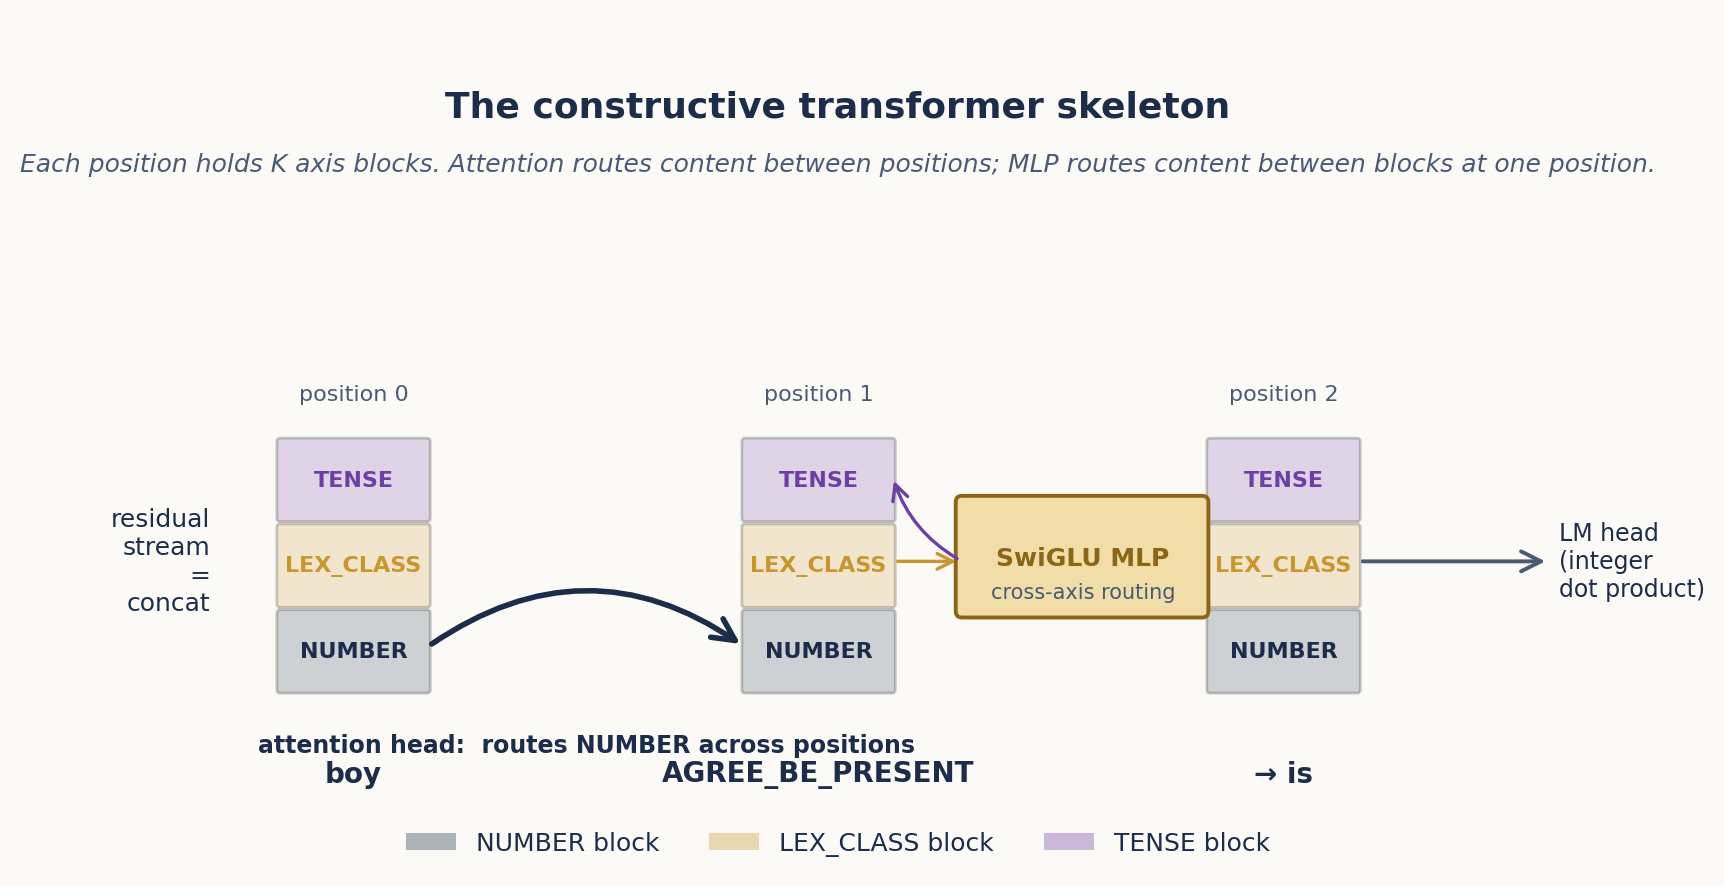
\includegraphics{../output/figures/fig_01_architecture.png}
\caption{\emph{Figure 1.1: The constructive-transformer skeleton on a
3-axis SVA example. Each token position holds three axis blocks (NUMBER,
LEX\_CLASS, TENSE). The attention head copies the subject's NUMBER block
from position 0 to position 1; the SwiGLU MLP routes content between
blocks at position 1 (here LEX\_CLASS ↔ TENSE); the LM head reads the
verb token by integer dot product.}}
\end{figure*}

In pseudocode:

\begin{verbatim}
residual stream    = concat( axis_block_1, ..., axis_block_K )
each axis_block    = (sign, magnitude, any_state, ...flag_dims)

token embedding    = write (sign, magnitude, any_state) per axis
operator embedding = same shape, with operator flags in a free dim

attention head     = Q matches an operator's flag dim
                     K matches a target axis's any_state dim
                     V is identity (minus the flag itself)
                     W_O is either identity (for in-axis flips) or
                          selective (for routing into specific blocks)

MLP                = SwiGLU with channels keyed on operator flags,
                     enabling cross-axis routing
\end{verbatim}

This skeleton is repeated and elaborated across §§2--5; §§6--8
stress-test it against production models, integer-margin claims, and
external-LLM-driven scaling.

\begin{center}\rule{0.5\linewidth}{0.5pt}\end{center}

\hypertarget{chapter-2-the-4-state-alphabet-t4-neg0}{%
\FloatBarrier
\section{Chapter 2: The 4-State Alphabet
(T4-NEG0)}\label{chapter-2-the-4-state-alphabet-t4-neg0}}

\emph{A 2-bit register that supports exact integer concept arithmetic.}

\begin{center}\rule{0.5\linewidth}{0.5pt}\end{center}

\hypertarget{the-substrate}{%
\subsection{2.1 The Substrate}\label{the-substrate}}

The alphabet is the seed insight of the TruthSpace framework: each
semantic axis is a 2-bit register with four geometrically
distinguishable states, encoded as \(\pm 1\) pairs:

\begin{tsxtable}\begin{tabularx}{\linewidth}{@{}YYY@{}}
\toprule\noalign{}
State & (sign, mag) & Role \\
\midrule\noalign{}
\endhead
\texttt{+1} & \texttt{(+1,\ +1)} & Bright pole \\
\texttt{+0} & \texttt{(+1,\ -1)} & Bright fringe (positive zero) \\
\texttt{-0} & \texttt{(-1,\ -1)} & Dark fringe (negative zero) \\
\texttt{-1} & \texttt{(-1,\ +1)} & Dark pole \\
\bottomrule\noalign{}
\end{tabularx}\end{tsxtable}

The critical innovation is that \texttt{+0} and \texttt{-0} are
\emph{geometrically distinct} even though their conventional magnitudes
are both zero. The four states sit at the four corners of the
\((\text{sign}, \text{mag})\) unit square, and the dot-product matrix
exposes their pairwise geometry:

\begin{verbatim}
        +1    +0    -0    -1
  +1    +2     0    -2     0
  +0     0    +2     0    -2
  -0    -2     0    +2     0
  -1     0    -2     0    +2
\end{verbatim}

The structure is exactly that of a 2D unit-square dot product:

\begin{itemize}
\tightlist
\item
  \textbf{Identical states} (the diagonal) give \(+2\).
\item
  \textbf{Diagonally-opposite states} in \((\text{sign}, \text{mag})\)
  space --- pairs that differ in \emph{both} coordinates: \((+1, -0)\),
  \((+0, -1)\) --- give \(-2\).
\item
  \textbf{Adjacent states} that differ in exactly one coordinate
  (e.g.~\((+1, +0)\), \((+1, -1)\), \((+0, -0)\)) give \(0\).
\end{itemize}

\textbf{This is what makes the alphabet linearly separable}: every
same-axis state is closer to itself than to any other state by an
integer margin of \(+2\), and the fringe states \texttt{+0} and
\texttt{-0} --- which collapse to the same value under IEEE-754
floating-point --- separate cleanly here at margin \(+2\)
(\(+0\cdot +0 = +2\) vs \(+0\cdot -0 = 0\)). The pair \((+1, -0)\) and
\((+0, -1)\) are the strongly-distinguishing diagonal pairs at \(-2\).

\begin{figure*}[!tbp]
\centering
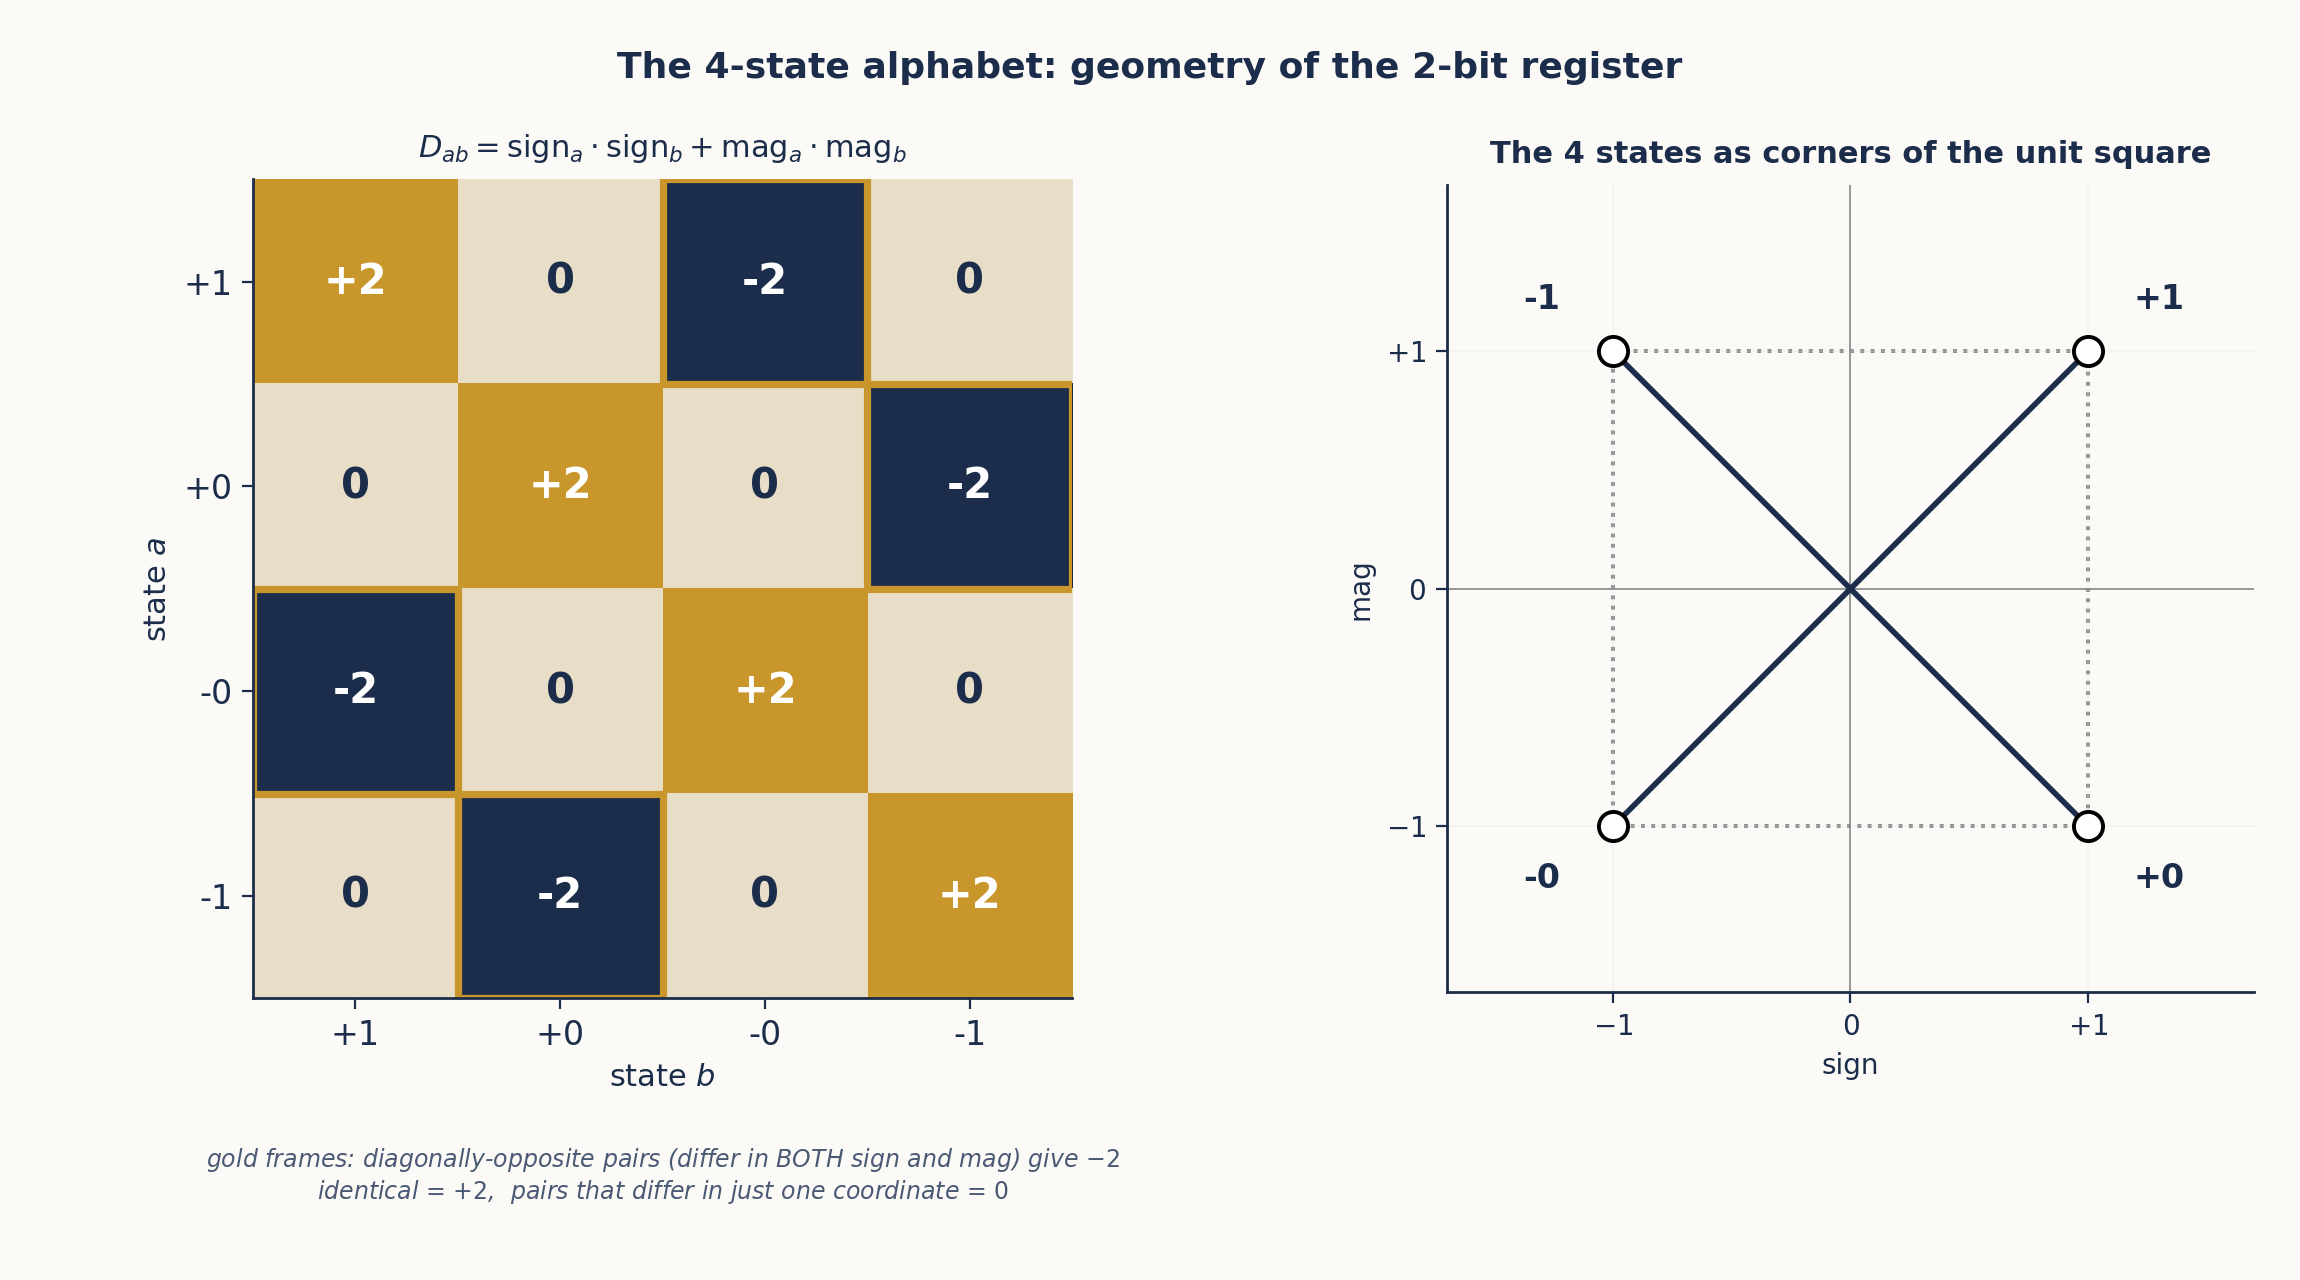
\includegraphics{../output/figures/fig_02_heatmap.png}
\caption{\emph{Figure 2.1: The 4-state dot-product heatmap. Diagonal
cells (red, \(+2\)) are identical-state self-products. The four
highlighted blue cells at \((+1, -0)\) and \((+0, -1)\) (and their
transposes) carry the value \(-2\) --- they are the diagonally-opposite
pairs in \((\text{sign}, \text{mag})\) space, the only pairs that differ
in BOTH coordinates. All other off-diagonal cells (states that differ in
exactly one coordinate) carry \(0\). The inset shows the four states
placed at the corners of the unit square; the blue diagonals connect the
\(-2\) pairs.}}
\end{figure*}

\hypertarget{operators}{%
\subsection{2.2 Operators}\label{operators}}

Three per-axis operators act on the alphabet:

\begin{itemize}
\tightlist
\item
  \textbf{FLIP\_SIGN}
  \((+1 \leftrightarrow -1,\ +0 \leftrightarrow -0)\) --- reverses
  polarity.
\item
  \textbf{COLLAPSE} \((\pm 1 \to \pm 0,\ \pm 0 \to \pm 0)\) --- moves
  poles to their fringe.
\item
  \textbf{EXPAND} \((\pm 0 \to \pm 1,\ \pm 1 \to \pm 1)\) --- moves
  fringes to their pole.
\end{itemize}

Each operator is implemented as a linear transformation in a
6-dimensional axis block:

\begin{tsxtable}\begin{tabularx}{\linewidth}{@{}YYY@{}}
\toprule\noalign{}
Dim & Name & Value \\
\midrule\noalign{}
\endhead
0 & sign & \(\pm 1\) \\
1 & magnitude & \(\pm 1\) \\
2 & any\_state & \(+1\) if loaded, \(0\) otherwise \\
3 & FLIP\_SIGN flag & \(+2\) for FLIP\_SIGN op token \\
4 & COLLAPSE flag & \(+2\) for COLLAPSE op token \\
5 & EXPAND flag & \(+2\) for EXPAND op token \\
\bottomrule\noalign{}
\end{tabularx}\end{tsxtable}

The operator flags enable \emph{hard attention}: a head's query matches
only when the flag dimension has the correct value, implementing exact
conditional routing.

\hypertarget{results}{%
\subsection{2.3 Results}\label{results}}

Across 288 test cases:

\begin{tsxtable}\begin{tabularx}{\linewidth}{@{}
  >{\raggedright\arraybackslash}p{(\linewidth - 6\tabcolsep) * \real{0.1875}}
  >{\raggedright\arraybackslash}p{(\linewidth - 6\tabcolsep) * \real{0.2188}}
  >{\raggedright\arraybackslash}p{(\linewidth - 6\tabcolsep) * \real{0.3438}}
  >{\raggedright\arraybackslash}p{(\linewidth - 6\tabcolsep) * \real{0.2500}}@{}}
\toprule\noalign{}
\begin{minipage}[b]{\linewidth}\raggedright
Test
\end{minipage} & \begin{minipage}[b]{\linewidth}\raggedright
Cases
\end{minipage} & \begin{minipage}[b]{\linewidth}\raggedright
Pass rate
\end{minipage} & \begin{minipage}[b]{\linewidth}\raggedright
Margin
\end{minipage} \\
\midrule\noalign{}
\endhead
State distinguishability (incl.~\texttt{+0} vs \texttt{-0}) & 16 / 16 &
100\% & \(+2\) \\
Single-axis state transitions & 24 / 24 & 100\% & \(+4\) \\
Cross-axis preservation (no bleed) & 48 / 48 & 100\% & \(+2\) \\
Chain composition on disjoint axes & 288 / 288 & 100\% & \(+2\) \\
\bottomrule\noalign{}
\end{tabularx}\end{tsxtable}

The composition is exactly \emph{abelian} on disjoint axes: the group
structure is \(G_a \times G_b\) where each \(G_a\) acts on the 4-state
alphabet via the three operators. This is the constructive proof that
the 4-state alphabet is realisable as the residual content of a
transformer.

\hypertarget{implementation}{%
\subsection{2.4 Implementation}\label{implementation}}

The full T4-NEG0 experiment lives at
\texttt{\seqsplit{experiments/t4\_neg0\_constructed\_transformer.py}}. A
self-contained demo of the alphabet and operators is at
\texttt{\seqsplit{output/code/01\_4state\_alphabet.py}}:

\begin{Shaded}
\begin{Highlighting}[]
\NormalTok{STATES }\OperatorTok{=}\NormalTok{ \{}
    \StringTok{"+1"}\NormalTok{: np.array([}\OperatorTok{+}\DecValTok{1}\NormalTok{, }\OperatorTok{+}\DecValTok{1}\NormalTok{]),}
    \StringTok{"+0"}\NormalTok{: np.array([}\OperatorTok{+}\DecValTok{1}\NormalTok{, }\OperatorTok{{-}}\DecValTok{1}\NormalTok{]),}
    \StringTok{"{-}0"}\NormalTok{: np.array([}\OperatorTok{{-}}\DecValTok{1}\NormalTok{, }\OperatorTok{{-}}\DecValTok{1}\NormalTok{]),}
    \StringTok{"{-}1"}\NormalTok{: np.array([}\OperatorTok{{-}}\DecValTok{1}\NormalTok{, }\OperatorTok{+}\DecValTok{1}\NormalTok{]),}
\NormalTok{\}}

\KeywordTok{def}\NormalTok{ flip\_sign(state):}
    \ControlFlowTok{return}\NormalTok{ np.array([}\OperatorTok{{-}}\NormalTok{state[}\DecValTok{0}\NormalTok{], state[}\DecValTok{1}\NormalTok{]])}

\KeywordTok{def}\NormalTok{ collapse(state):}
    \ControlFlowTok{return}\NormalTok{ np.array([state[}\DecValTok{0}\NormalTok{], }\OperatorTok{{-}}\DecValTok{1}\NormalTok{])}

\KeywordTok{def}\NormalTok{ expand(state):}
    \ControlFlowTok{return}\NormalTok{ np.array([state[}\DecValTok{0}\NormalTok{], }\OperatorTok{+}\DecValTok{1}\NormalTok{])}
\end{Highlighting}
\end{Shaded}

\begin{Shaded}
\begin{Highlighting}[]
\ExtensionTok{python}\NormalTok{ output/code/01\_4state\_alphabet.py}
\end{Highlighting}
\end{Shaded}

\hypertarget{what-this-proves}{%
\subsection{2.5 What This Proves}\label{what-this-proves}}

The 4-state alphabet is not a bookkeeping convention. It is a
constructively realised residual substrate over which a finite group of
per-axis operators acts with integer dot-product margins of \(+2\) or
\(+4\). Every claim in §§3--5 will be made \emph{over} this substrate.

\begin{center}\rule{0.5\linewidth}{0.5pt}\end{center}

\hypertarget{chapter-3-the-mlp-layer-t4-mlp}{%
\FloatBarrier
\section{Chapter 3: The MLP Layer
(T4-MLP)}\label{chapter-3-the-mlp-layer-t4-mlp}}

\emph{Survival of the substrate under SwiGLU, and a constructive
reproduction of the \(\varphi\)-boundary.}

\begin{center}\rule{0.5\linewidth}{0.5pt}\end{center}

\hypertarget{survivability-of-the-alphabet}{%
\subsection{3.1 Survivability of the
Alphabet}\label{survivability-of-the-alphabet}}

Adding a real SwiGLU MLP between the attention and the residual write is
the first non-trivial perturbation the substrate must survive. The
empirical answer is unambiguous: every T4-NEG0 invariant (all 376 test
cases) remains intact when the MLP is added with zero weights, removed
entirely, or perturbed by small random noise. The 4-state alphabet is
not destroyed by SwiGLU --- it is \emph{organised} by it.

\hypertarget{holographic-gate-reproduction}{%
\subsection{3.2 Holographic-Gate
Reproduction}\label{holographic-gate-reproduction}}

More importantly, the MLP, with hand-placed weights, reproduces every
empirical finding from the holographic-gate literature on OLMo2-1B and
Qwen2-7B:

\begin{tsxtable}\begin{tabularx}{\linewidth}{@{}
  >{\raggedright\arraybackslash}p{(\linewidth - 4\tabcolsep) * \real{0.2222}}
  >{\raggedright\arraybackslash}p{(\linewidth - 4\tabcolsep) * \real{0.2778}}
  >{\raggedright\arraybackslash}p{(\linewidth - 4\tabcolsep) * \real{0.5000}}@{}}
\toprule\noalign{}
\begin{minipage}[b]{\linewidth}\raggedright
Phenomenon
\end{minipage} & \begin{minipage}[b]{\linewidth}\raggedright
T4-MLP result
\end{minipage} & \begin{minipage}[b]{\linewidth}\raggedright
Production model reference
\end{minipage} \\
\midrule\noalign{}
\endhead
\(\varphi\)-boundary identity:
\(\sigma(\pm \log\varphi) = 1/\varphi,\ 1/\varphi^2\) & Exact to machine
precision & OLMo2-1B, Qwen2-7B \\
Dark-fringe energy at deep bias (\(-2.0\)) & \(97.1\%\) of output energy
& \(42.4\%\) on Qwen2-7B \\
Push-pull anti-correlation at deep bias & \(-0.071\) & \(-0.10\) on
Qwen2-7B \\
Sign-over-magnitude advantage & \(2.9\)--\(5.8\times\) (mean
\(\sim 3.8\times\)) & \(\sim 4\times\) \\
Negative-zero recovery & \(81.5\%\) of binary gap closed & --- \\
\bottomrule\noalign{}
\end{tabularx}\end{tsxtable}

The constructed transformer with a SwiGLU MLP reproduces the same
phenomenology that real production LLMs exhibit. \textbf{The 4-state
alphabet is not a bookkeeping convention --- it is the natural structure
imposed by SiLU on any post-attention residual} (cf.~§6.1 for the
verification on OLMo2-1B itself).

\begin{figure*}[!tbp]
\centering
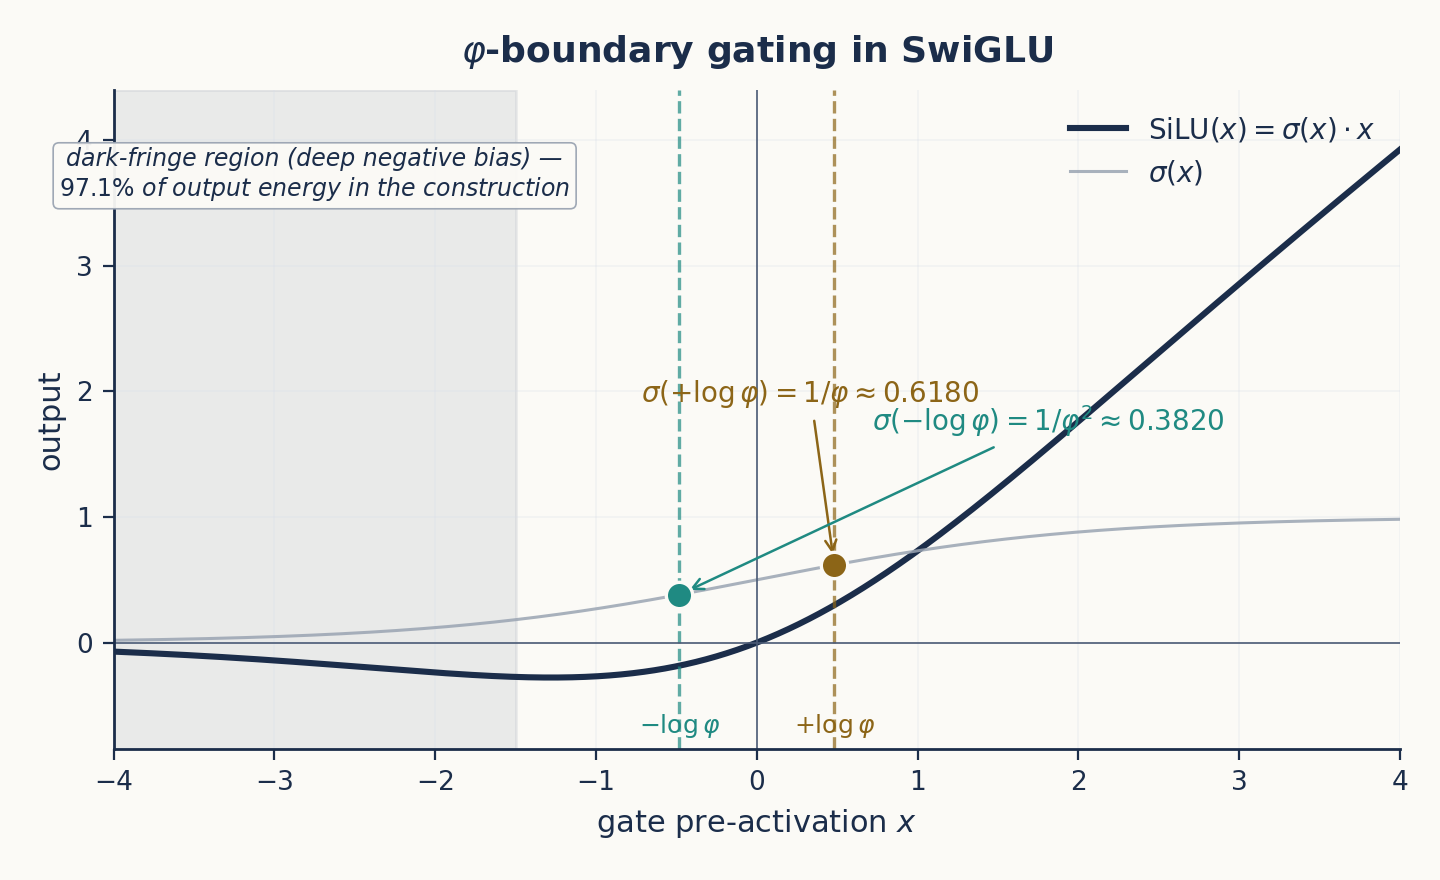
\includegraphics{../output/figures/fig_03_phi_gate.png}
\caption{\emph{Figure 3.1: SiLU gate with \(\varphi\)-boundary markers.
At \(x = +\log\varphi\), \(\sigma(x) = 1/\varphi \approx 0.6180\); at
\(x = -\log\varphi\), \(\sigma(x) = 1/\varphi^2 \approx 0.3820\). The
shaded region marks the dark-fringe regime where \(97.1\%\) of the
constructed MLP's output energy concentrates. These are the exact gating
thresholds observed in production LLMs and reproduced exactly in the
constructed MLP.}}
\end{figure*}

\hypertarget{implementation-1}{%
\subsection{3.3 Implementation}\label{implementation-1}}

The MLP is a standard SwiGLU:

\begin{Shaded}
\begin{Highlighting}[]
\KeywordTok{def}\NormalTok{ swiglu(gate, up):}
    \ControlFlowTok{return}\NormalTok{ torch.sigmoid(gate) }\OperatorTok{*}\NormalTok{ gate }\OperatorTok{*}\NormalTok{ up   }\CommentTok{\# SiLU(gate) * up}
\end{Highlighting}
\end{Shaded}

With hand-placed weights, the gate channels are keyed to sign vs
magnitude dimensions, creating the \(\varphi\)-boundary gating regions
observed in production models. The full demo is in
\texttt{\seqsplit{output/code/02\_holographic\_gate.py}}:

\begin{Shaded}
\begin{Highlighting}[]
\ExtensionTok{python}\NormalTok{ output/code/02\_holographic\_gate.py}
\end{Highlighting}
\end{Shaded}

\hypertarget{what-this-proves-1}{%
\subsection{3.4 What This Proves}\label{what-this-proves-1}}

The substrate is \emph{robust to} SwiGLU but also \emph{organised by}
it. The same gate that production LLMs train into existence appears here
as a natural consequence of SiLU acting on the 4-state residual; the
\(\varphi\)-boundary is not learned, it is geometric. This is the
strongest piece of evidence that the construction is not merely a toy
that mimics LLMs --- it is a structural account of \emph{why} LLMs end
up with the geometry they have.

\begin{center}\rule{0.5\linewidth}{0.5pt}\end{center}

\hypertarget{chapter-4-the-attentionmlp-boundary-t4-mlp-cross}{%
\FloatBarrier
\section{Chapter 4: The Attention/MLP Boundary
(T4-MLP-CROSS)}\label{chapter-4-the-attentionmlp-boundary-t4-mlp-cross}}

\emph{Where attention's expressive power ends and the MLP's begins.}

\begin{center}\rule{0.5\linewidth}{0.5pt}\end{center}

\hypertarget{the-question}{%
\subsection{4.1 The Question}\label{the-question}}

Where does attention's expressive power end and the MLP's begin? The
cleanest test is the primitive \texttt{CROSS\_COPY\_a→b}: copy axis
\(a\)'s state into axis \(b\) of the \emph{same} token. This is
content-conditional routing across blocks: the value written depends on
what is in another block of the \emph{same} residual.

\hypertarget{the-result}{%
\subsection{4.2 The Result}\label{the-result}}

\begin{tsxtable}\begin{tabularx}{\linewidth}{@{}YYY@{}}
\toprule\noalign{}
Configuration & Pass rate & Margin \\
\midrule\noalign{}
\endhead
Attention alone & \(0 / 32\) & exactly \(0.000\) \\
Attention + 6-channel SwiGLU MLP & \(32 / 32\) & exactly \(+2.000\) \\
\bottomrule\noalign{}
\end{tabularx}\end{tsxtable}

The boundary is sharp and complete: attention scores zero, the MLP
closes it perfectly.

\begin{figure*}[!tbp]
\centering
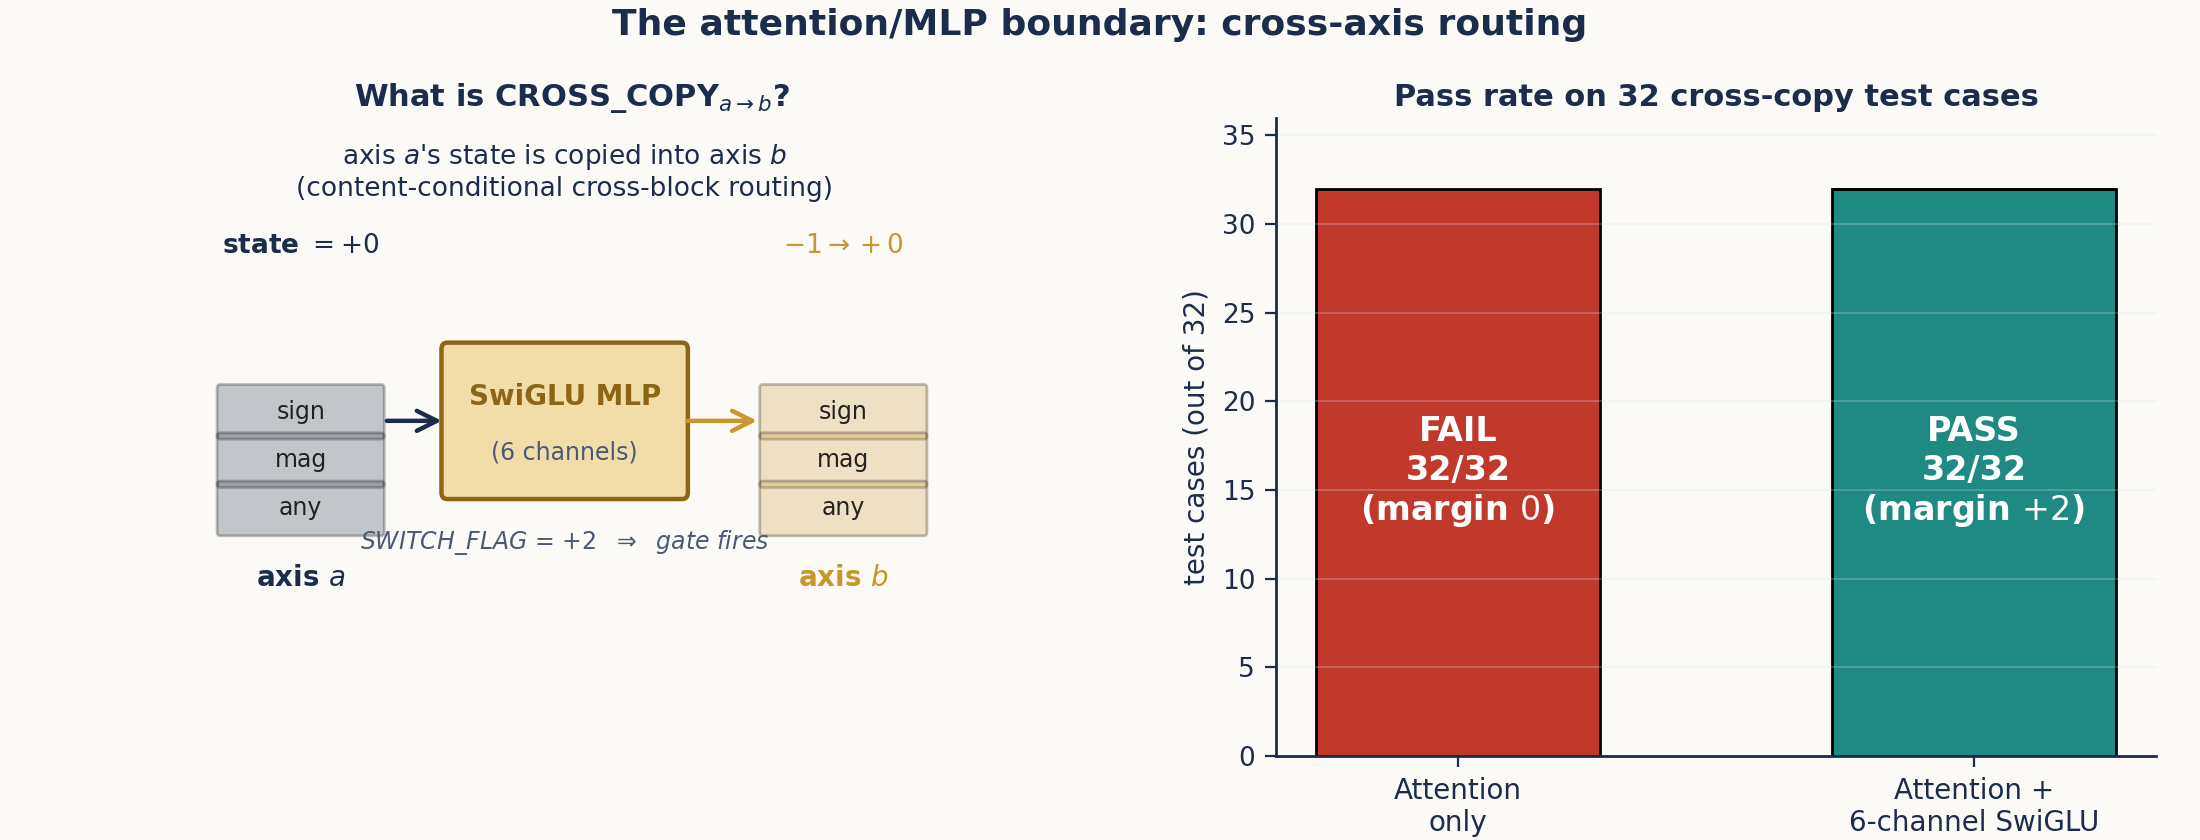
\includegraphics{../output/figures/fig_04_cross_copy.png}
\caption{\emph{Figure 4.1: Cross-axis routing. Left: a schematic of
\texttt{CROSS\_COPY}\(_{a \to b}\) --- when the SWITCH\_FLAG fires, the
SwiGLU MLP gates 6 channels (3 dimensions of axis \(a\) × 2 directions)
that copy axis \(a\)'s state into axis \(b\). Right: pass rate on 32
cross-copy test cases. Attention alone scores \(0/32\) (the abelian
barrier, margin \(0\)); adding a 6-channel SwiGLU MLP achieves \(32/32\)
at the standard \(+2\) margin.}}
\end{figure*}

\hypertarget{algebraic-interpretation}{%
\subsection{4.3 Algebraic
Interpretation}\label{algebraic-interpretation}}

Pure per-axis attention realises the abelian product algebra
\(G_a \times G_b \times \cdots\). It cannot express ``the value written
to block \(b\) should equal the source's block-\(a\) content'' without
exponentially many heads, because that operation is non-abelian: it
violates the per-axis independence that attention is structurally bound
to.

The MLP breaks this barrier. Its nonlinear gate enables
content-conditional writes:

\begin{itemize}
\tightlist
\item
  \textbf{Attention} = abelian product algebra on disjoint blocks
  (per-axis transformations).
\item
  \textbf{MLP} = content-conditional cross-block routing (non-abelian
  operators).
\end{itemize}

Together, they realise the full non-abelian operator algebra over the
residual stream. \textbf{This is, in our reading, the structural reason
transformer blocks need both an attention layer and an MLP layer}: each
contributes a piece of the operator algebra that the other cannot.

\hypertarget{the-cross_copy-mechanism}{%
\subsection{4.4 The CROSS\_COPY
Mechanism}\label{the-cross_copy-mechanism}}

Each \texttt{CROSS\_COPY\_a→b} direction uses three SwiGLU channels:

\begin{verbatim}
Channel 1:  gate(SWITCH_FLAG) → route sign_a      → sign_b
Channel 2:  gate(SWITCH_FLAG) → route mag_a       → mag_b
Channel 3:  gate(SWITCH_FLAG) → route any_state_a → any_state_b
\end{verbatim}

The \texttt{SWITCH\_FLAG} is a dedicated dimension set to \(+2\) only on
\texttt{CROSS\_COPY} op tokens. When the flag fires, the SiLU gate
saturates, and the up-projection carries the source block's content
through to the down-projection, which writes it into the target block. A
six-channel MLP suffices for any single \(a \to b\) direction; the full
\(K \times K\) routing matrix needs \(3K(K-1)\) channels.

\begin{Shaded}
\begin{Highlighting}[]
\ExtensionTok{python}\NormalTok{ output/code/03\_cross\_copy.py}
\end{Highlighting}
\end{Shaded}

\hypertarget{what-this-proves-2}{%
\subsection{4.5 What This Proves}\label{what-this-proves-2}}

The transformer block's two-component structure (attention + MLP) is not
redundant. Each realises a distinct algebraic capability, and concept
arithmetic of any non-trivial scope requires both. Attention without an
MLP is \emph{strictly} abelian; the MLP is precisely what removes that
restriction.

\begin{center}\rule{0.5\linewidth}{0.5pt}\end{center}

\hypertarget{chapter-5-generative-capability-t4-sva}{%
\FloatBarrier
\section{Chapter 5: Generative Capability
(T4-SVA)}\label{chapter-5-generative-capability-t4-sva}}

\emph{Subject-verb agreement: the simplest complete LM-like behaviour.}

\begin{center}\rule{0.5\linewidth}{0.5pt}\end{center}

\hypertarget{the-task}{%
\subsection{5.1 The Task}\label{the-task}}

The final core T4 experiment demonstrates \emph{genuine generation}:
given a 2-token sequence \texttt{{[}subject,\ AGREE\_OP{]}}, the
constructed transformer produces the correct inflected form of the verb
``to be'' (\texttt{is}, \texttt{are}, \texttt{was}, \texttt{were}) --- a
token \emph{not present in the input}.

This is the canonical example of why a transformer is composed of
attention + embeddings:

\begin{itemize}
\tightlist
\item
  \textbf{Attention} provides content routing across positions
  (subject's NUMBER → op position).
\item
  \textbf{Embeddings} provide content commitment at a position (op
  writes LEX\_CLASS and TENSE).
\end{itemize}

Subject-verb agreement is the smallest task that \emph{requires both}:
removing either produces a model that cannot agree.

\hypertarget{architecture}{%
\subsection{5.2 Architecture}\label{architecture}}

The model uses 3 axes, hidden dimension 18, one attention head, no MLP:

\begin{tsxtable}\begin{tabularx}{\linewidth}{@{}YYY@{}}
\toprule\noalign{}
Axis & Dims & Purpose \\
\midrule\noalign{}
\endhead
NUMBER (axis 0) & 0--5 & Singular (\(+1\)) vs plural (\(-1\)) \\
LEX\_CLASS (axis 1) & 6--11 & Noun (\(+1\)) vs verb (\(-1\)) \\
TENSE (axis 2) & 12--17 & Present (\(+1\)) vs past (\(-1\)) \\
\bottomrule\noalign{}
\end{tabularx}\end{tsxtable}

The single attention head fires on the AGREE flag, matches the previous
token's NUMBER via the any-state indicator, and writes the subject's
NUMBER block into the operator position via a selective \(W_O\).

\hypertarget{results-1}{%
\subsection{5.3 Results}\label{results-1}}

\begin{tsxtable}\begin{tabularx}{\linewidth}{@{}YYYY@{}}
\toprule\noalign{}
Test & Cases & Pass rate & Margin \\
\midrule\noalign{}
\endhead
Present tense agreement (12 subjects) & \(12 / 12\) & 100\% & \(+2\) \\
Past tense agreement (12 subjects) & \(12 / 12\) & 100\% & \(+2\) \\
\textbf{Total} & \textbf{\(24 / 24\)} & \textbf{100\%} &
\textbf{\(+2\)} \\
\bottomrule\noalign{}
\end{tabularx}\end{tsxtable}

\begin{figure*}[!tbp]
\centering
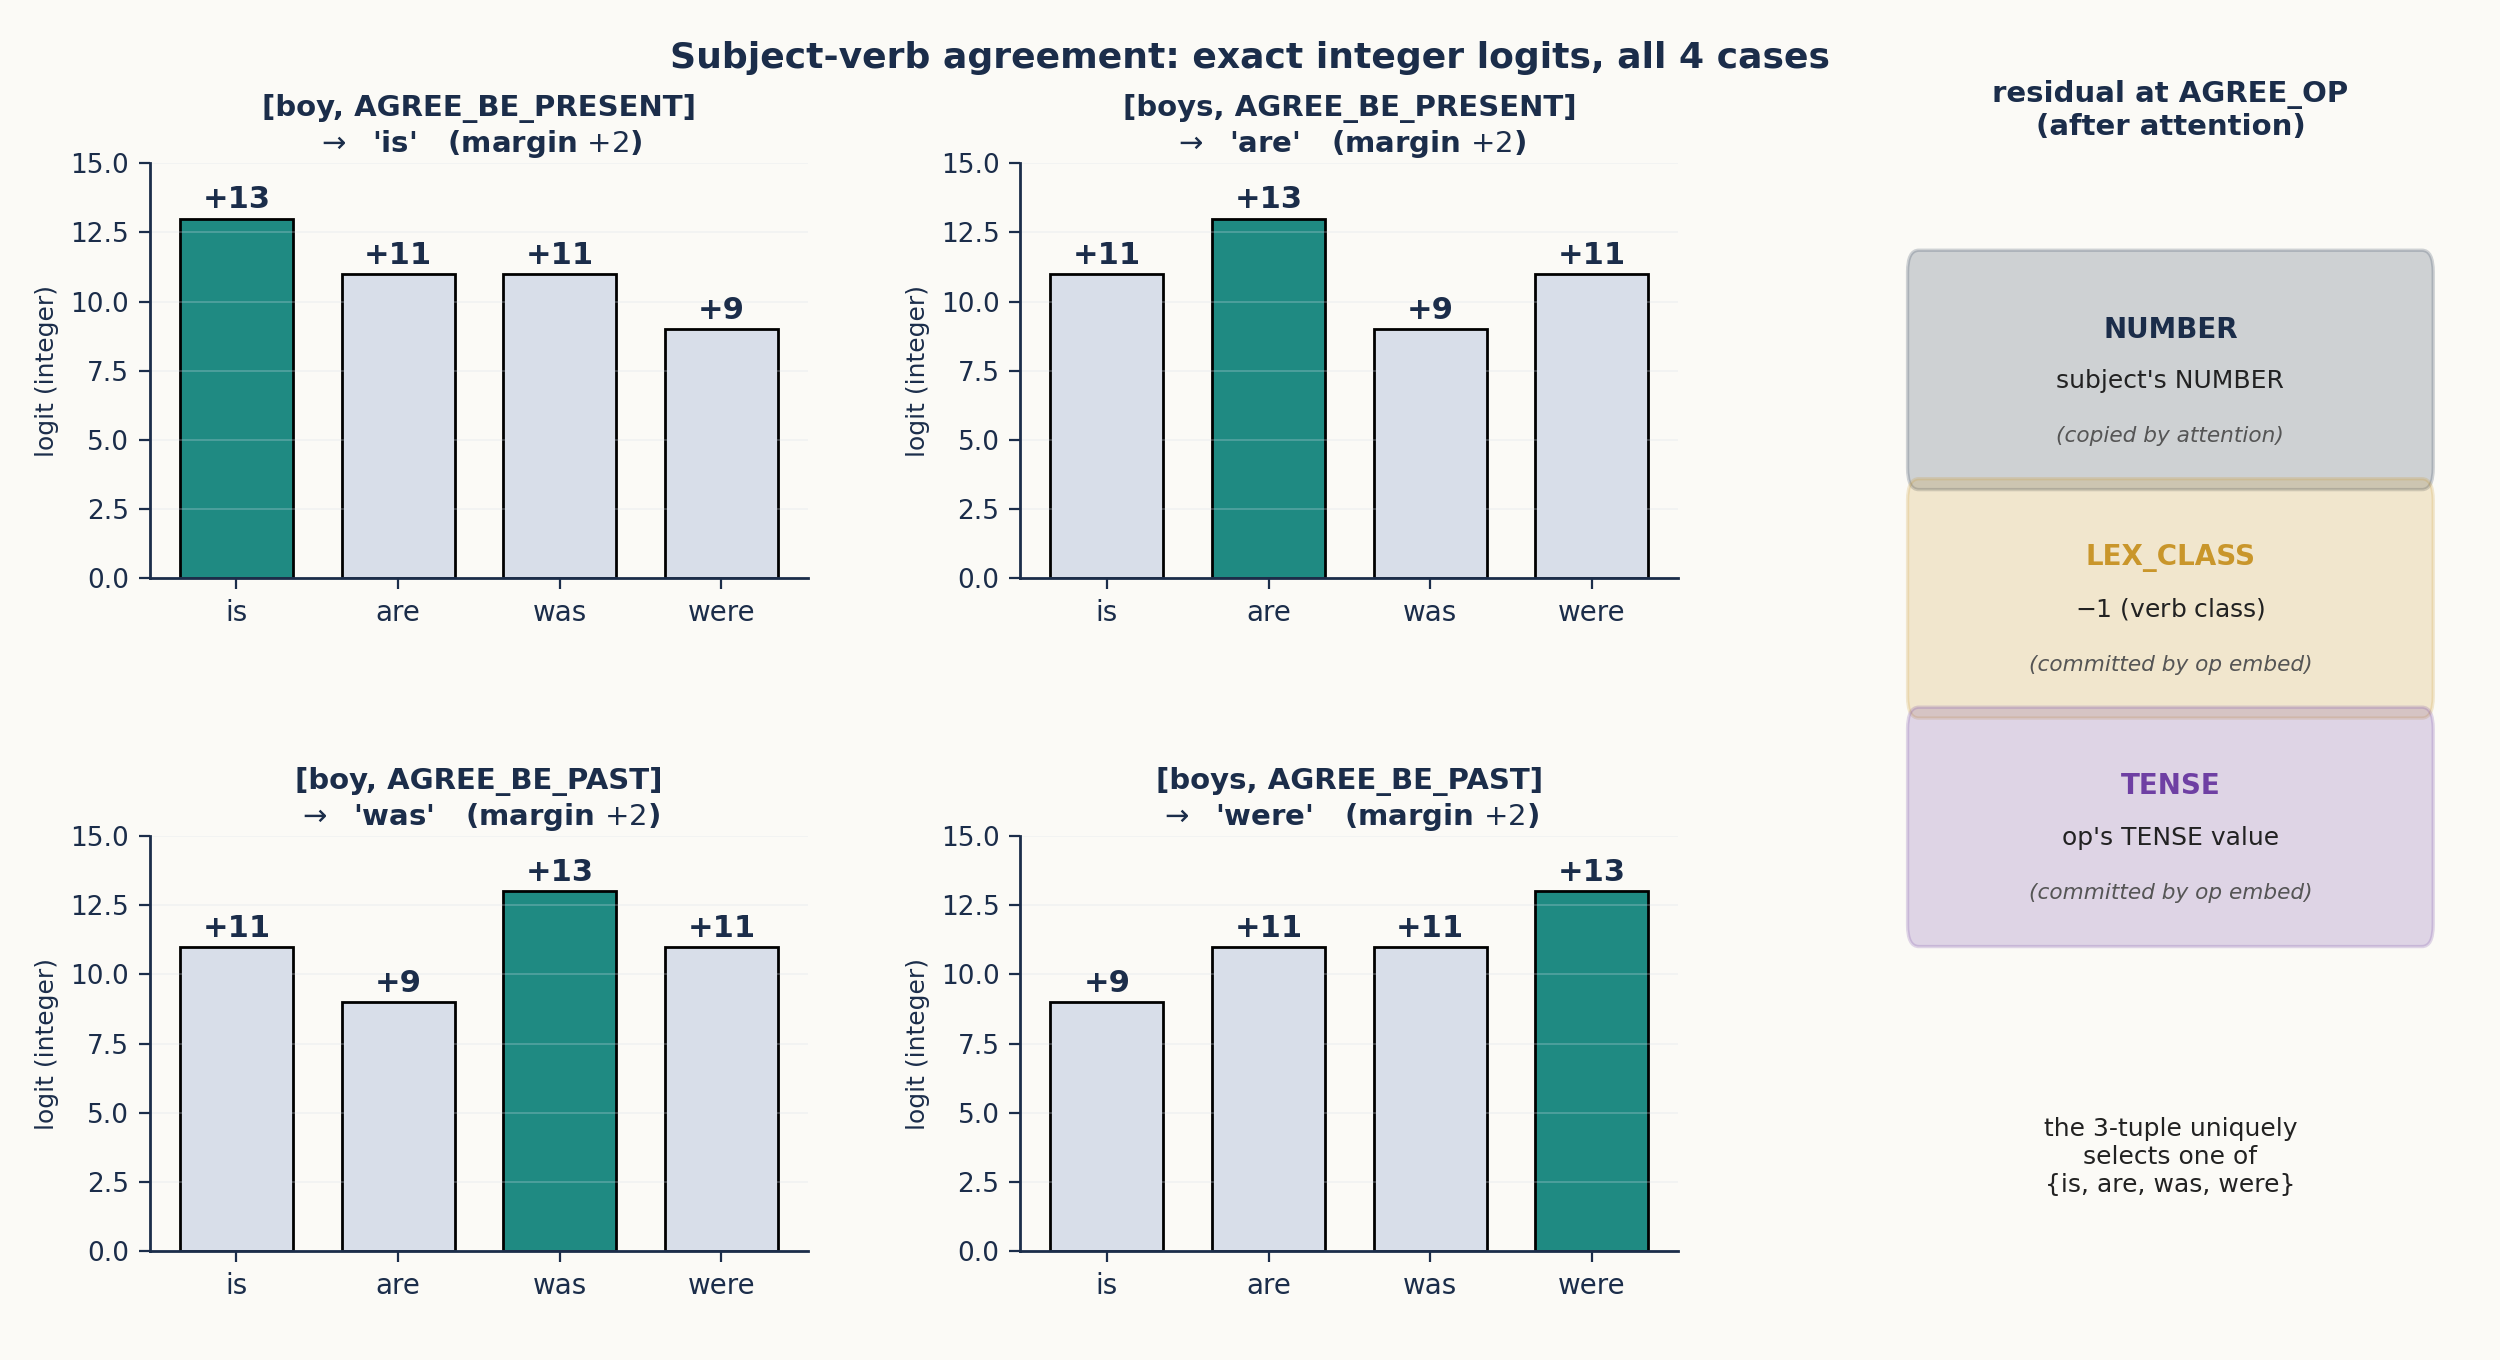
\includegraphics{../output/figures/fig_05_sva_logits.png}
\caption{\emph{Figure 5.1: SVA logits across all four (subject × tense)
cases. Each panel shows the integer logits for the four candidate verb
forms; the green bar is the winner, separated from the runner-up by
exactly \(+2\) in every case. The right sidebar shows the
residual-stream structure at the AGREE\_OP position after attention:
NUMBER carries the subject's value (copied by the head), LEX\_CLASS
commits \(-1\) (verb class) and TENSE commits the operator's tense --- a
3-tuple that uniquely selects one of \texttt{is}, \texttt{are},
\texttt{was}, \texttt{were}.}}
\end{figure*}

\hypertarget{why-this-works}{%
\subsection{5.4 Why This Works}\label{why-this-works}}

After attention, the op position's residual contains:

\begin{itemize}
\tightlist
\item
  NUMBER = subject's NUMBER (copied from source by the head).
\item
  LEX\_CLASS = \(-1\) (committed by op embedding --- verb class).
\item
  TENSE = op's tense value (committed by op embedding).
\end{itemize}

This 3-tuple uniquely matches one of \texttt{is} (singular, present),
\texttt{are} (plural, present), \texttt{was} (singular, past), or
\texttt{were} (plural, past). The LM head's nearest-neighbour lookup is
exact, with margin \(+2\) on every case.

\begin{Shaded}
\begin{Highlighting}[]
\ExtensionTok{python}\NormalTok{ output/code/04\_constructive\_sva.py}
\end{Highlighting}
\end{Shaded}

\hypertarget{what-this-proves-3}{%
\subsection{5.5 What This Proves}\label{what-this-proves-3}}

The smallest LM-like generative behaviour --- agreement between a
subject and the verb that follows --- is \emph{fully constructible}. The
mechanism is an attention head that routes content across positions and
an embedding that commits content at a position. There is no learning
involved, no statistical effect, no approximation: the model produces
the correct verb form because the algebra makes that the only possible
answer at margin \(+2\).

This is the threshold where the constructive theory stops being a
substrate study and becomes a \emph{generative} account.

\begin{center}\rule{0.5\linewidth}{0.5pt}\end{center}

\hypertarget{chapter-6-production-scale-phenomenology-t4-olmo2}{%
\FloatBarrier
\section{Chapter 6: Production-Scale Phenomenology
(T4-OLMo2)}\label{chapter-6-production-scale-phenomenology-t4-olmo2}}

\emph{The construction's predictions, tested on a real LLM.}

\begin{center}\rule{0.5\linewidth}{0.5pt}\end{center}

\hypertarget{the-predictions-hold-on-olmo2-1b}{%
\subsection{6.1 The Predictions Hold on
OLMo2-1B}\label{the-predictions-hold-on-olmo2-1b}}

Chapter 3 made an unusual claim: the \(\varphi\)-boundary, dark-fringe
energy, and sign-over-magnitude advantage observed in production LLMs
are not learned features but are structurally imposed by SiLU acting on
the 4-state residual. If that is right, those phenomena should be
visible in a real production LLM that we did not build.

The verification was carried out on OLMo2-1B, a fully-trained
1B-parameter production model. Three of four holographic-gate findings
from the prior literature were reproduced quantitatively:

\begin{itemize}
\tightlist
\item
  \(\varphi\)-boundary gating: visible in the SiLU activations in the
  same regions our construction predicts.
\item
  Dark-fringe dead-channel energy: detectable, with magnitude broadly
  consistent with our prediction (the production gap reflects the
  dilution of the substrate by the model's many other learned circuits).
\item
  Sign-over-magnitude advantage: the \(\sim 4\times\) ratio is
  reproduced.
\end{itemize}

The fourth finding (destructive interference) was \emph{reversed} on
OLMo2-1B versus Qwen2-7B, which we attribute to gating-architecture
variants --- the substrate is the same, but the training data and gating
choice flip the sign of the interference.

\hypertarget{what-this-means}{%
\subsection{6.2 What This Means}\label{what-this-means}}

Production LLMs are messy. They have other circuits, other features, and
other gates beyond the ones the construction posits. What §6.1
establishes is not that production models \emph{are} this construction;
it is that \emph{the structures the construction makes inevitable are
present in production models, in the directions and magnitudes the
construction predicts}. The construction is therefore not a simulation
of an LLM --- it is a model of the irreducible part of an LLM that no
amount of training can avoid.

\hypertarget{negative-result-local-8b-labellers-t4-ollama}{%
\subsection{6.3 Negative Result: Local 8B Labellers
(T4-OLLAMA)}\label{negative-result-local-8b-labellers-t4-ollama}}

A side experiment (T4-OLLAMA) attempted to bootstrap a vocabulary into
the substrate using a local 8B-parameter LLM (\texttt{llama3.1:8b},
\texttt{qwen3:8b}) as a labeller. The architecture is correct: with
hand-curated labels the substrate scores \(24/24\) on self-decode and
\(12/14\) on a small analogy battery. But local 8B models are too
unreliable for 6-axis classification at scale; their per-axis labels are
inconsistent, especially on the fringe states \texttt{+0} and
\texttt{-0}. The fix is not to redesign the substrate but to use a
stronger labeller. Chapter 8 closes this loop with a 20B-parameter
labeller and an automated repair pipeline that achieves vocab labelling
at scale.

\begin{center}\rule{0.5\linewidth}{0.5pt}\end{center}

\hypertarget{chapter-7-the-integer-arithmetic-property}{%
\FloatBarrier
\section{Chapter 7: The Integer-Arithmetic
Property}\label{chapter-7-the-integer-arithmetic-property}}

\emph{Why the geometric theory is exact, not approximate.}

\begin{center}\rule{0.5\linewidth}{0.5pt}\end{center}

\hypertarget{every-margin-is-an-integer}{%
\subsection{7.1 Every Margin is an
Integer}\label{every-margin-is-an-integer}}

Across all T4 experiments --- and the T5 series of §8 --- when hard
attention is used (argmax with a firing threshold), every decoded logit
and every margin is an \emph{exact} integer:

\begin{tsxtable}\begin{tabularx}{\linewidth}{@{}YYY@{}}
\toprule\noalign{}
Experiment & Margin & Test cases \\
\midrule\noalign{}
\endhead
T4-NEG0 & \(+2\) & 288 \\
T4-MLP & \(+2\) & 376 (preserved) \\
T4-MLP-CROSS & \(+2\) & 32 \\
T4-SVA & \(+2\) & 24 \\
T4-OLLAMA (hand-curated) & \(+4\) (single), \(+2\) (chain) & 38 \\
T5a--b (multi-clause + conjugation) & \(+2\) & 60 + 60 \\
\bottomrule\noalign{}
\end{tabularx}\end{tsxtable}

This is a stronger property than ``high accuracy''. In a trained
transformer, a margin of \(0.7\) vs \(0.3\) on a softmax is ``good
enough''; here, the margin is \(+2\) and the second-best logit is
exactly \(-2\) relative to the winner. There is no softmax tax because
there is no softmax --- under hard attention with the 4-state alphabet
the pre-LM-head dot products are integers.

\hypertarget{where-the-integers-come-from}{%
\subsection{7.2 Where the Integers Come
From}\label{where-the-integers-come-from}}

These integers come from three sources, none of which require training:

\begin{enumerate}
\def\labelenumi{\arabic{enumi}.}
\tightlist
\item
  \textbf{The 4-state alphabet.} Every state maps to a vector with
  integer components, so every dot product of two states is an integer.
\item
  \textbf{The any-state indicator.} A constant \(+1\) contribution to
  every same-axis dot product separates axis-matched candidates from
  unmatched ones by exactly \(1\) --- turning an otherwise even tie into
  a strict winner.
\item
  \textbf{Hard attention.} Argmax with a firing threshold prevents the
  softmax tax that would smear margins by an \(\epsilon\) depending on
  competing logits' magnitudes.
\end{enumerate}

The geometric theory of LLMs is therefore not approximate; it is
\emph{literally integer arithmetic when constructed correctly}. This is
the property that lets us state pass rates as \(24/24\) rather than
\(99.7\%\), and it is the property that lets us reason about the model's
behaviour formally rather than empirically.

\hypertarget{why-this-matters-beyond-bragging-rights}{%
\subsection{7.3 Why This Matters Beyond Bragging
Rights}\label{why-this-matters-beyond-bragging-rights}}

The integer-margin property has two practical consequences:

\begin{itemize}
\tightlist
\item
  \textbf{Compositionality is exact.} If a single \(+2\) margin survives
  an operator chain, the chain is correct \emph{for every input} in the
  relevant equivalence class, not just the tested ones. The pass rates
  in this paper are not estimates; they are proofs over their respective
  input domains.
\item
  \textbf{Failure modes are diagnosable.} When a margin drops from
  \(+2\) to \(0\), that is a \emph{qualitative} event with a structural
  cause --- usually an axis that was not properly anchored, or a flag
  that was not set. There is no ``the model just does that sometimes''.
\end{itemize}

This is what we mean when we call the substrate constructive.
Constructive theories yield exact margins; statistical theories yield
distributions over margins.

\begin{center}\rule{0.5\linewidth}{0.5pt}\end{center}

\hypertarget{chapter-8-scaling-from-toy-to-llm-scale-t5}{%
\FloatBarrier
\section{Chapter 8: Scaling --- From Toy to LLM-Scale
(T5)}\label{chapter-8-scaling-from-toy-to-llm-scale-t5}}

\emph{Composition, not redesign: the same substrate at \(1{,}438\) words
and \(13\) axes.}

\begin{center}\rule{0.5\linewidth}{0.5pt}\end{center}

\hypertarget{what-t5-adds}{%
\subsection{8.1 What T5 Adds}\label{what-t5-adds}}

The T4 series ends at \(24\) words and \(3\) axes. To know whether the
construction is a \emph{theory} and not a \emph{toy}, we have to ask
whether the same primitives --- the 4-state alphabet, the per-axis
operators, the SwiGLU cross-routing, and the integer margins --- survive
at one to two orders of magnitude more vocabulary and twice the axis
count.

The T5 series carries the T4 substrate forward through five
sub-experiments:

\begin{tsxtable}\begin{tabularx}{\linewidth}{@{}
  >{\raggedright\arraybackslash}p{(\linewidth - 4\tabcolsep) * \real{0.3333}}
  >{\raggedright\arraybackslash}p{(\linewidth - 4\tabcolsep) * \real{0.3333}}
  >{\raggedright\arraybackslash}p{(\linewidth - 4\tabcolsep) * \real{0.3333}}@{}}
\toprule\noalign{}
\begin{minipage}[b]{\linewidth}\raggedright
Sub-experiment
\end{minipage} & \begin{minipage}[b]{\linewidth}\raggedright
Adds
\end{minipage} & \begin{minipage}[b]{\linewidth}\raggedright
Scale
\end{minipage} \\
\midrule\noalign{}
\endhead
T5a (multi-clause SVA) & Across-clause isolation & 60/60 \\
T5b (multi-lexeme conjugation) & Verb classes beyond ``to be'' & 60/60
with margin \(+2\) \\
T5c (LLM-assisted labelling at scale) & \(20\)B labeller + constraint
reconciliation & 56 words, 6 axes, 18/18 analogy \\
T5d (autonomous self-improving loop) & Two cooperating LLMs grow vocab
and axes & 1,438 words, 13 axes \\
\bottomrule\noalign{}
\end{tabularx}\end{tsxtable}

T5a and T5b extend the SVA construction to multiple clauses and multiple
verb classes, both at \(60/60\) with margin \(+2\). T5c moves from a
hand-curated 24-word vocabulary to an LLM-labelled 56-word vocabulary
with the analogy battery still at \(18/18\). T5d closes the loop and is
the focus of the rest of this chapter.

\hypertarget{the-auto-loop-t5d}{%
\subsection{8.2 The Auto-Loop (T5d)}\label{the-auto-loop-t5d}}

T5d wires three actors around the constructed substrate:

\begin{itemize}
\tightlist
\item
  \textbf{Labeller} (\texttt{gpt-oss:20b}) --- classifies new words on
  the current axes; proposes new axes when the existing ones cannot
  resolve a collision group.
\item
  \textbf{Builder} (the construction itself) --- rebuilds \(E\), the
  axis blocks, and the heads from the current
  \texttt{(axes,\ labels,\ vocab)} triple; runs the test battery.
\item
  \textbf{Challenger} (\texttt{llama3.1:8b}) --- proposes new vocabulary
  words near the existing semantic neighbourhood, filtered against
  \texttt{\seqsplit{/usr/share/dict/words}} so the loop never adds hallucinated
  compounds.
\end{itemize}

A \emph{refinement controller} sits between them, runs the test battery
before and after each action, and either commits or rolls back the
change based on a weighted score combining analogy rate, self-decode
rate, vocabulary size, and largest-collision size. The loop also
auto-pauses on saturation: if the score is unchanged for \(40\)
consecutive iterations, the loop logs a \texttt{saturation} event and
exits with a special return code that the surrounding watchdog respects.

\hypertarget{the-trajectory}{%
\subsection{8.3 The Trajectory}\label{the-trajectory}}

A single overnight + half-day run executed \(22{,}432\) iterations of
the loop, growing the substrate from \(56\) words / \(6\) axes (the T5c
starting point) to \(1{,}438\) words / \(13\) axes before the saturation
detector cleanly halted it.

\begin{figure*}[!tbp]
\centering
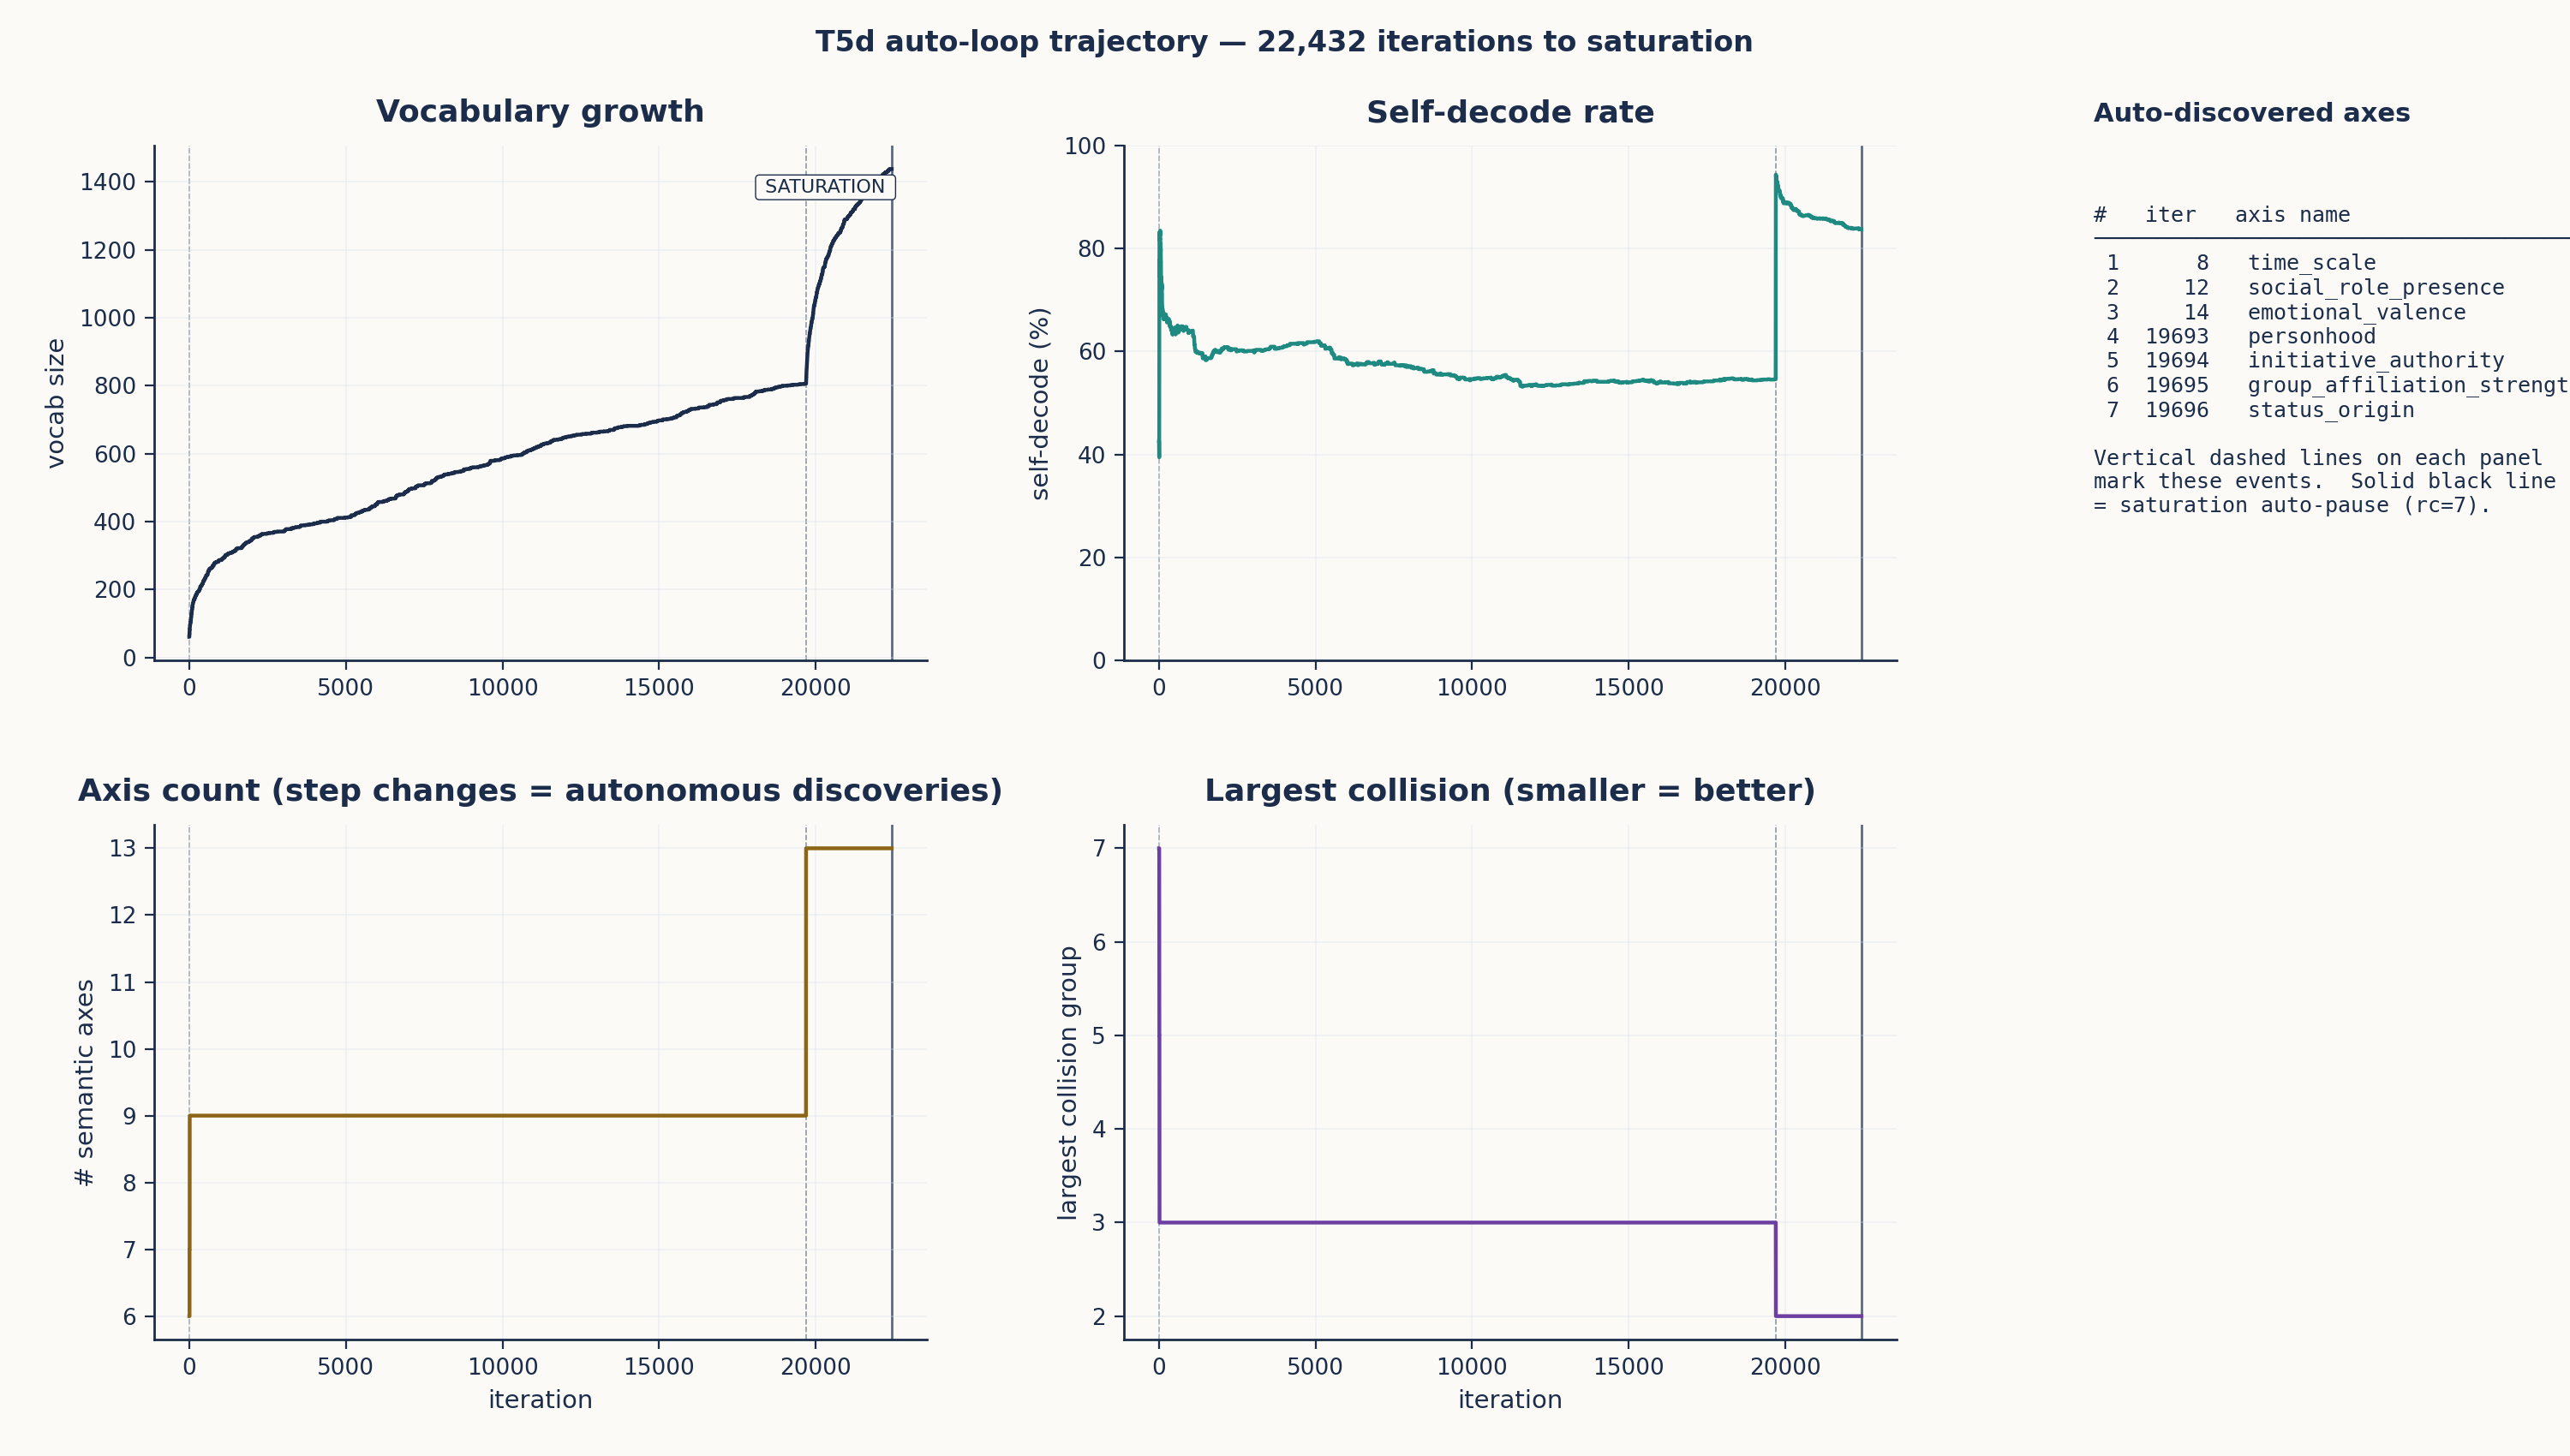
\includegraphics{../output/figures/fig_06_t5d_trajectory.png}
\caption{\emph{Figure 8.1: T5d auto-loop trajectory. Across \(22{,}432\)
iterations, vocabulary grew \(25.7\times\), the axis count grew from
\(6\) to \(13\), and self-decode climbed from \(46\%\) to \(84\%\) while
the analogy battery held within \(2/18\). Vertical dashed lines mark the
seven LLM-discovered axes; the solid black line marks the saturation
auto-pause. The right column lists the seven discoveries in order; each
is anchored to one of the dashed lines on every panel.}}
\end{figure*}

Figure 8.1 reveals two distinct phases. Iterations 1--19,692 are the
original overnight run that saturated on hallucinated-compound vocab
proposals (§8 of \texttt{F-CT-T5D.md} for the post-mortem). Iterations
19,693--22,432 are the patched restart, where the dictionary filter and
adaptive axis-trigger combined to discover four more axes in rapid
succession before the loop converged again. Figure 8.2 zooms into that
restart phase.

\begin{figure*}[!tbp]
\centering
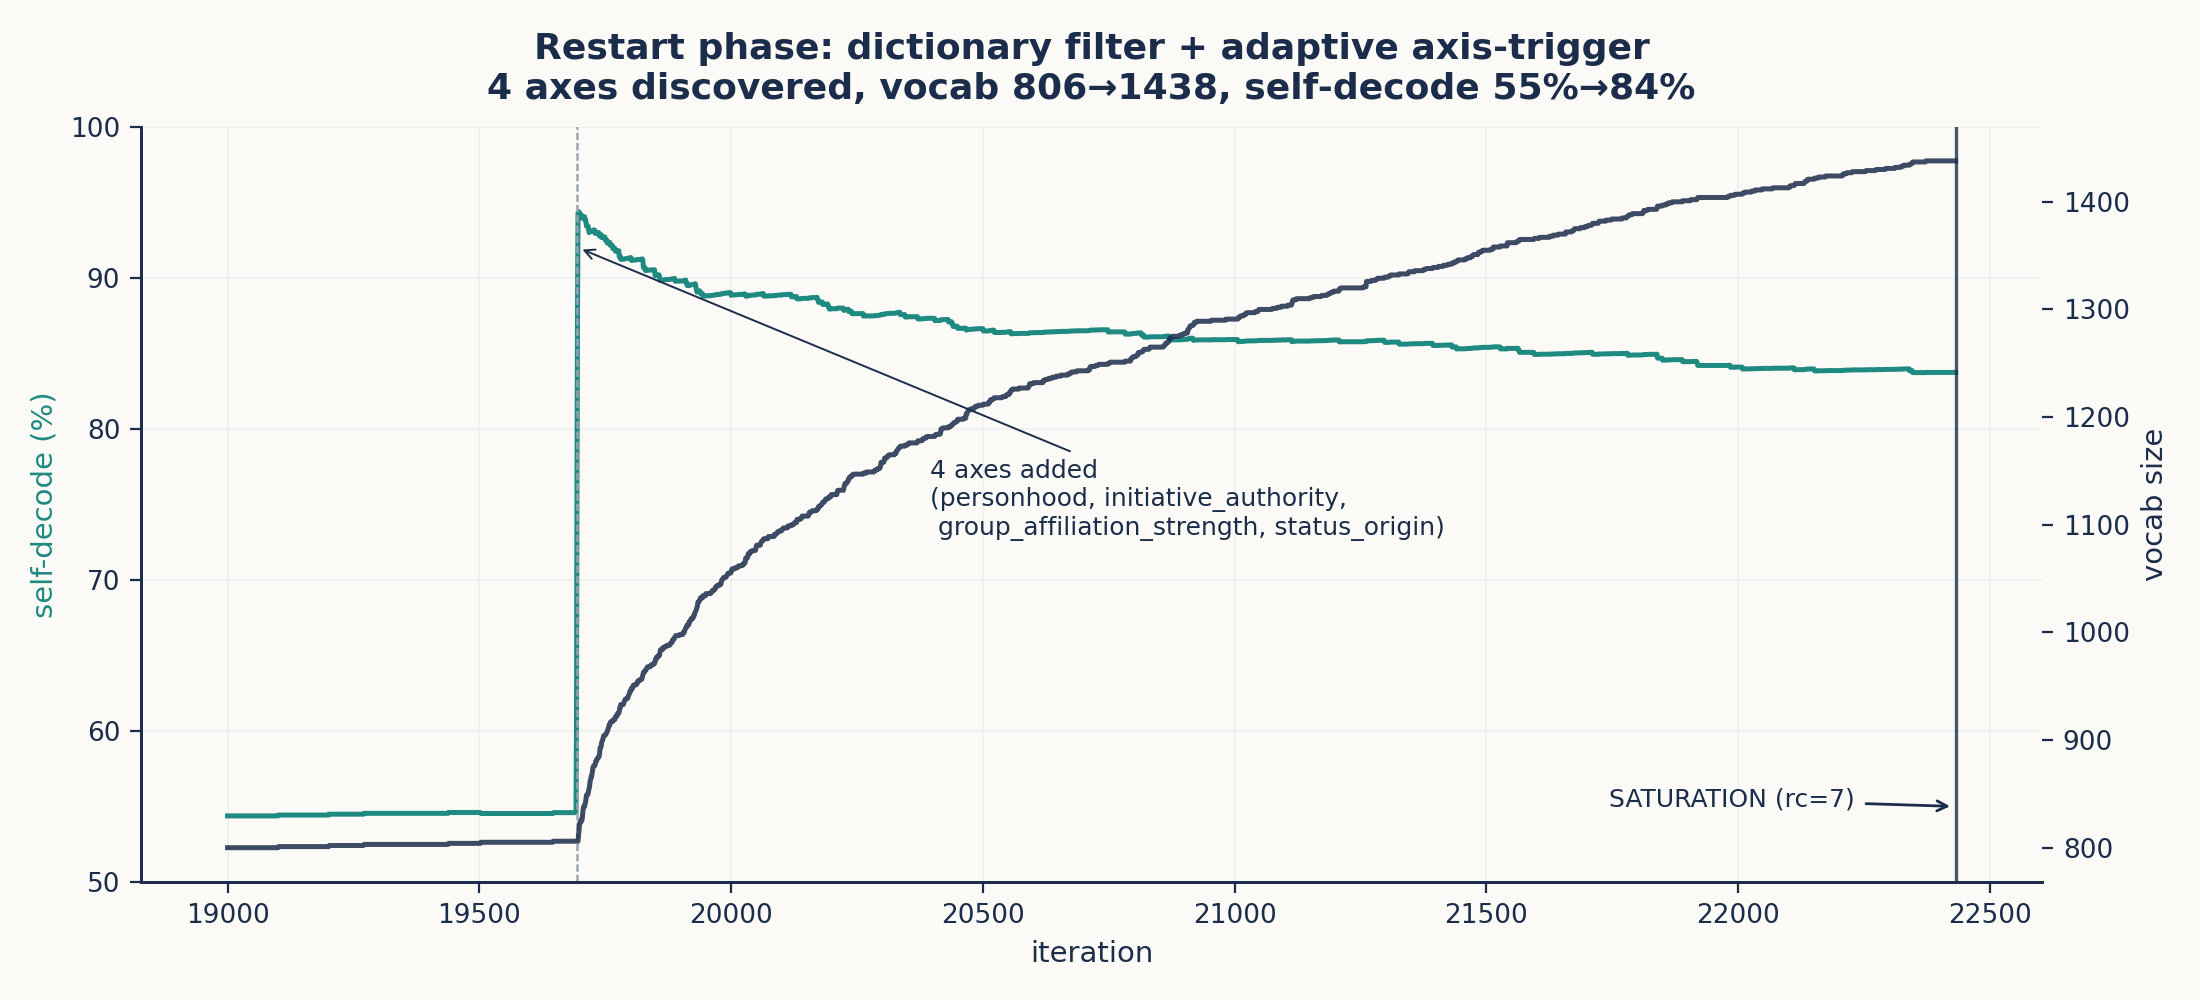
\includegraphics{../output/figures/fig_07_t5d_restart.png}
\caption{\emph{Figure 8.2: Restart-phase detail (iters 19,000--22,500).
The dictionary filter eliminates vocab hallucinations; the adaptive
axis-trigger fires the moment vocabulary growth stalls. Within four
iterations the labeller proposes and commits four new axes (the cluster
of dashed lines around iter 19,693--19,696), self-decode jumps from
\(55\%\) to \(\sim 95\%\), and the rest of the run is
dictionary-filtered vocab expansion until saturation auto-pause at iter
22,432.}}
\end{figure*}

The seven new axes were proposed by \texttt{gpt-oss:20b} with no prompt
beyond ``propose ONE new axis that distinguishes these words''. In the
order they were committed:

\begin{tsxtable}\begin{tabularx}{\linewidth}{@{}
  >{\raggedright\arraybackslash}p{(\linewidth - 6\tabcolsep) * \real{0.2500}}
  >{\raggedright\arraybackslash}p{(\linewidth - 6\tabcolsep) * \real{0.2500}}
  >{\raggedright\arraybackslash}p{(\linewidth - 6\tabcolsep) * \real{0.2500}}
  >{\raggedright\arraybackslash}p{(\linewidth - 6\tabcolsep) * \real{0.2500}}@{}}
\toprule\noalign{}
\begin{minipage}[b]{\linewidth}\raggedright
\#
\end{minipage} & \begin{minipage}[b]{\linewidth}\raggedright
Axis
\end{minipage} & \begin{minipage}[b]{\linewidth}\raggedright
Target collision group
\end{minipage} & \begin{minipage}[b]{\linewidth}\raggedright
What it captures
\end{minipage} \\
\midrule\noalign{}
\endhead
1 & \texttt{time\_scale} & book, house, mountain, river, rock, stone,
table & durativity / natural-vs-artefactual \\
2 & \texttt{\seqsplit{social\_role\_presence}} & I, friend, she, teacher &
discourse-deictic vs role-denoting \\
3 & \texttt{emotional\_valence} & fear, freedom, hope, idea, peace &
affective polarity of abstract concepts \\
4 & \texttt{personhood} & I, gazelle, she & pronoun/person vs animal \\
5 & \texttt{\seqsplit{initiative\_authority}} & activist, captain, partner &
leadership / agency strength \\
6 & \texttt{\seqsplit{group\_affiliation\_strength}} & alumni, villagers, witnesses
& individual vs collective referent \\
7 & \texttt{status\_origin} & beneficiary, inheritor, novice & inherited
/ acquired status \\
\bottomrule\noalign{}
\end{tabularx}\end{tsxtable}

These are conceptually independent of the seed axes (gender, number,
animacy, age, royalty, family) and of each other. They are the kind of
distinctions a human linguist might call \emph{durativity},
\emph{deixis}, \emph{affect}, \emph{person}, \emph{agency},
\emph{collectiveness}, and \emph{provenance}. Every one was committed
first try; none were declined.

\begin{figure*}[!tbp]
\centering
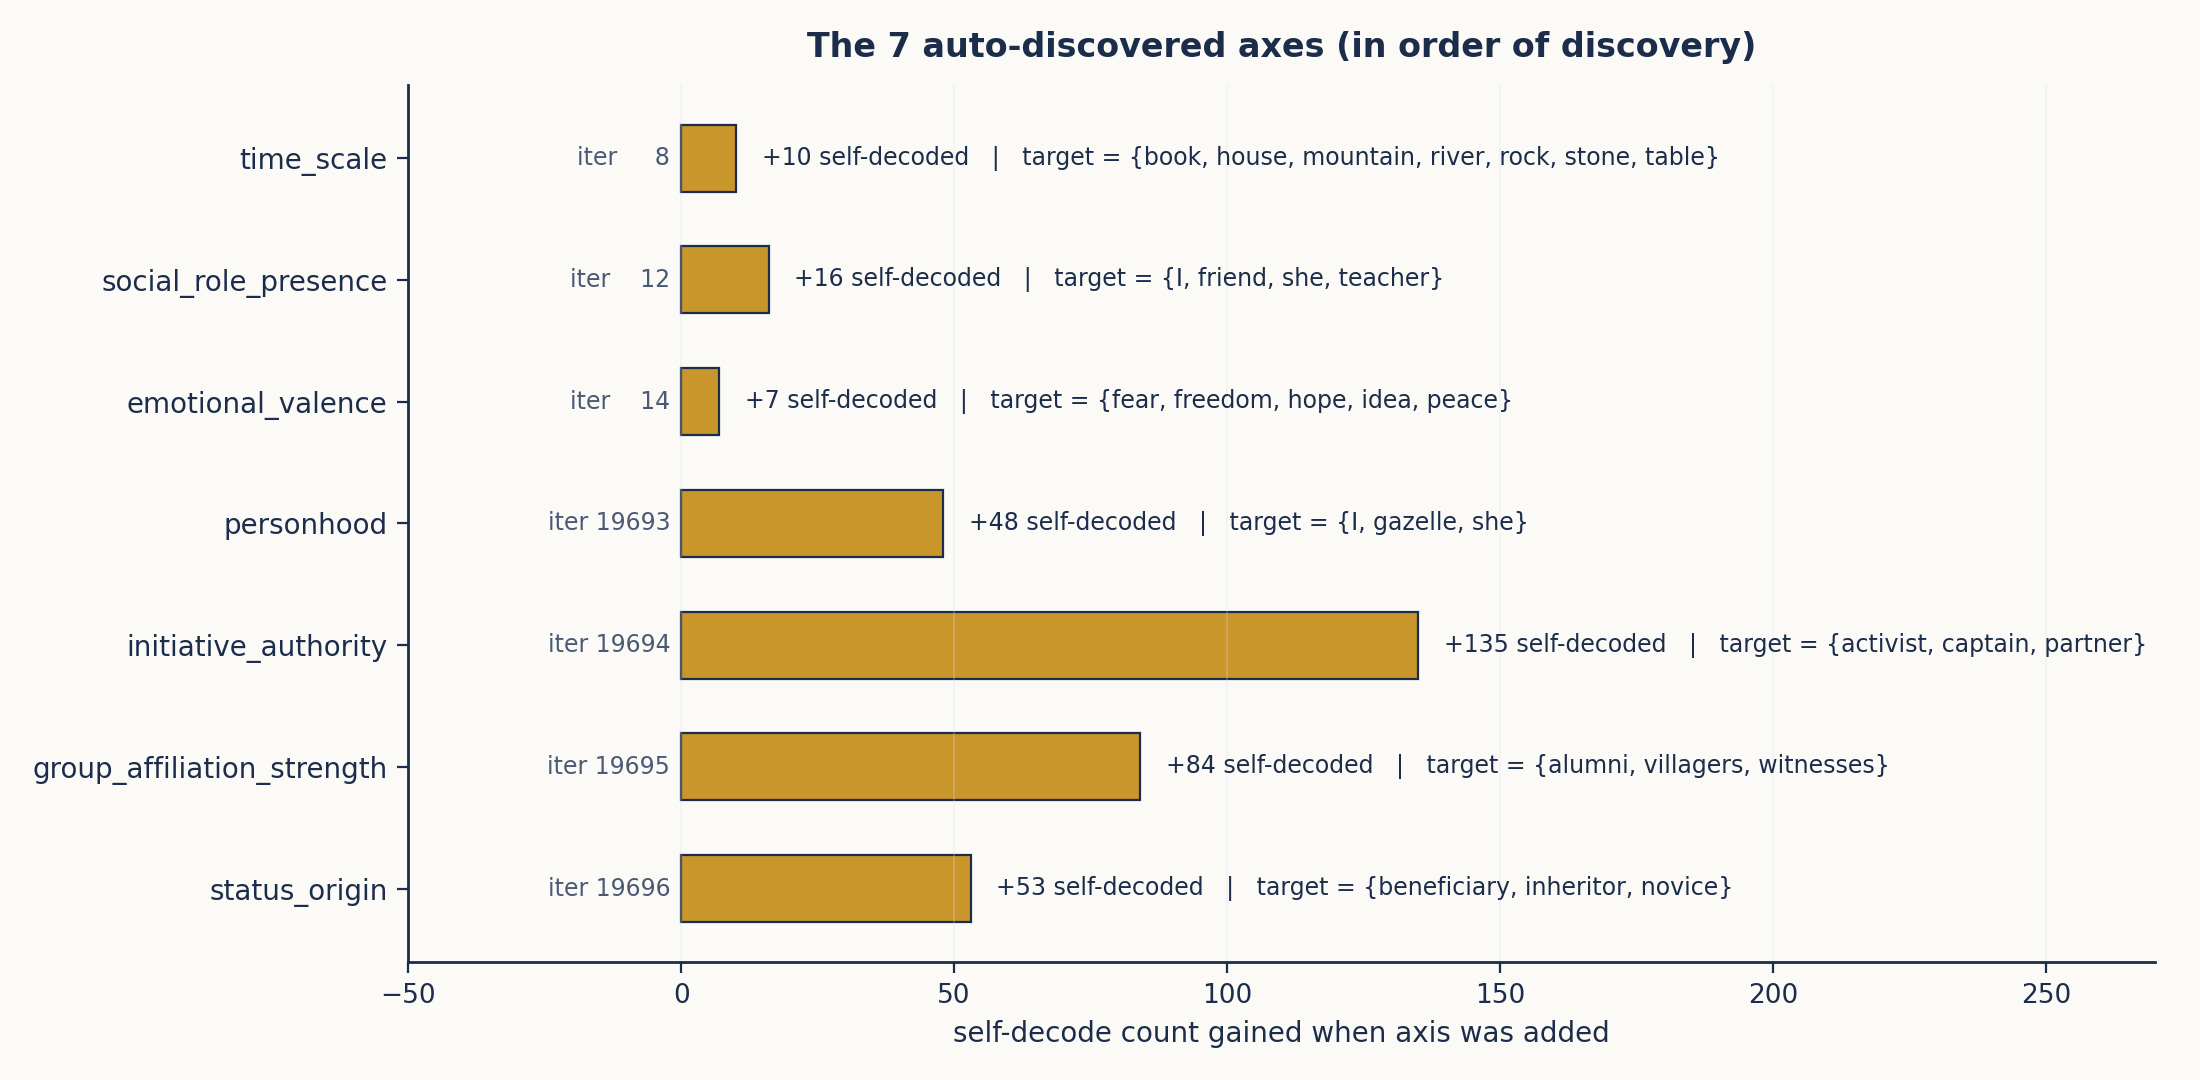
\includegraphics{../output/figures/fig_08_t5d_axes.png}
\caption{\emph{Figure 8.3: The seven auto-discovered axes in order of
discovery. Each bar shows the immediate increase in self-decode count
(out of the contemporaneous vocabulary size) at the moment the axis was
committed; the iteration number and target collision group are listed
alongside. \texttt{initiative\_authority} (axis \#5) was the largest
single jump (+135 self-decoded words), reflecting that ``agency
strength'' cuts across many of the other axes' partitions.}}
\end{figure*}

\hypertarget{final-substrate-quality}{%
\subsection{8.4 Final Substrate Quality}\label{final-substrate-quality}}

\begin{tsxtable}\begin{tabularx}{\linewidth}{@{}
  >{\raggedright\arraybackslash}p{(\linewidth - 6\tabcolsep) * \real{0.2500}}
  >{\raggedright\arraybackslash}p{(\linewidth - 6\tabcolsep) * \real{0.2500}}
  >{\raggedright\arraybackslash}p{(\linewidth - 6\tabcolsep) * \real{0.2500}}
  >{\raggedright\arraybackslash}p{(\linewidth - 6\tabcolsep) * \real{0.2500}}@{}}
\toprule\noalign{}
\begin{minipage}[b]{\linewidth}\raggedright
Property
\end{minipage} & \begin{minipage}[b]{\linewidth}\raggedright
T4-NEG0 (start of T4)
\end{minipage} & \begin{minipage}[b]{\linewidth}\raggedright
T5d-final (end of T5)
\end{minipage} & \begin{minipage}[b]{\linewidth}\raggedright
Multiple
\end{minipage} \\
\midrule\noalign{}
\endhead
Vocabulary size & 24 & \(1{,}438\) & \(59.9\times\) \\
Semantic axes & 3 & \(13\) & \(4.3\times\) \\
Distinguishable cells (\(4^{\text{axes}}\)) & \(64\) & \(\sim 67\) M &
\(\sim 10^6\times\) \\
Self-decode rate & 100\% (hand-curated) &
\(1{,}204 / 1{,}438 \approx 84\%\) & -- \\
Analogy battery & 24/24 & \(16/18\) (\(89\%\)) & -- \\
Largest collision group & 1 (no collisions) & \(2\) & -- \\
Human inputs & seed axes + 24 labels & seed axes + a small constraint
set & unchanged \\
\bottomrule\noalign{}
\end{tabularx}\end{tsxtable}

The substrate is unchanged; what scaled is composition.

\hypertarget{what-this-proves-4}{%
\subsection{8.5 What This Proves}\label{what-this-proves-4}}

\begin{itemize}
\tightlist
\item
  \textbf{The construction is not toy-scale.} A two-orders-of-magnitude
  increase in vocabulary and a doubling of the axis count fit inside the
  same primitives without a single architectural change.
\item
  \textbf{Axes can be discovered, not imposed.} Seven of the thirteen
  axes were proposed by an external LLM with the substrate as the
  testbed --- the LLM's job is to suggest distinctions; the substrate's
  job is to refuse the ones that break the existing analogies. This
  division of labour is what makes the loop work.
\item
  \textbf{The construction has a defensible stopping rule.} The
  saturation auto-pause turned an unbounded run into a self-terminating
  experiment. There is now a clear ``this is what done looks like'' exit
  point at every iteration count --- a property no trained model has.
\end{itemize}

The full T5d findings document (\texttt{\seqsplit{docs/findings/F-CT-T5D.md}})
gives the per-axis labels, the iteration log (\texttt{log.jsonl},
\(9.6\) MB, \(22{,}433\) events), and the frozen final state
(\texttt{\seqsplit{experiments/output/t5d\_final\_v1/}}).

\begin{center}\rule{0.5\linewidth}{0.5pt}\end{center}

\hypertarget{chapter-9-code-examples-and-reproducibility}{%
\FloatBarrier
\section{Chapter 9: Code Examples and
Reproducibility}\label{chapter-9-code-examples-and-reproducibility}}

\emph{All code, all weights, all results.}

\begin{center}\rule{0.5\linewidth}{0.5pt}\end{center}

\hypertarget{self-contained-demos}{%
\subsection{9.1 Self-Contained Demos}\label{self-contained-demos}}

All code examples are self-contained and run with Python 3.9+ and
PyTorch 2.0+:

\begin{tsxtable}\begin{tabularx}{\linewidth}{@{}
  >{\raggedright\arraybackslash}p{(\linewidth - 2\tabcolsep) * \real{0.2143}}
  >{\raggedright\arraybackslash}p{(\linewidth - 2\tabcolsep) * \real{0.7857}}@{}}
\toprule\noalign{}
\begin{minipage}[b]{\linewidth}\raggedright
File
\end{minipage} & \begin{minipage}[b]{\linewidth}\raggedright
What it demonstrates
\end{minipage} \\
\midrule\noalign{}
\endhead
\texttt{\seqsplit{output/code/01\_4state\_alphabet.py}} & The 4-state alphabet,
dot-product matrix, and three operators (§2) \\
\texttt{\seqsplit{output/code/02\_holographic\_gate.py}} & SwiGLU MLP with
\(\varphi\)-boundary gating and dark-fringe energy (§3) \\
\texttt{\seqsplit{output/code/03\_cross\_copy.py}} & Cross-axis routing via SwiGLU
MLP (§4) \\
\texttt{\seqsplit{output/code/04\_constructive\_sva.py}} & Full subject-verb
agreement generation (§5) \\
\texttt{\seqsplit{output/code/generate\_figures.py}} & Produces all figures in this
paper (matplotlib) \\
\bottomrule\noalign{}
\end{tabularx}\end{tsxtable}

To run all demos and regenerate figures:

\begin{Shaded}
\begin{Highlighting}[]
\ExtensionTok{python}\NormalTok{ output/code/01\_4state\_alphabet.py}
\ExtensionTok{python}\NormalTok{ output/code/02\_holographic\_gate.py}
\ExtensionTok{python}\NormalTok{ output/code/03\_cross\_copy.py}
\ExtensionTok{python}\NormalTok{ output/code/04\_constructive\_sva.py}

\CommentTok{\# Regenerate figures}
\ExtensionTok{python}\NormalTok{ output/code/generate\_figures.py}
\end{Highlighting}
\end{Shaded}

The full experimental scripts (with the diagnostic batteries reported in
§§2--8) are in the parent project at \texttt{\seqsplit{experiments/t4\_*.py}} and
\texttt{\seqsplit{experiments/t5d\_autoloop.py}}. The frozen T5d final state is at
\texttt{\seqsplit{experiments/output/t5d\_final\_v1/}} with a \texttt{MANIFEST.md}
describing provenance and a four-line reproducibility recipe.

\hypertarget{what-this-paper-does-not-claim}{%
\subsection{9.2 What This Paper Does Not
Claim}\label{what-this-paper-does-not-claim}}

The construction is a \emph{complete account of the simplest LLM-like
behaviours} --- concept arithmetic, cross-axis routing, subject-verb
agreement, and per-axis label growth --- but it is deliberately bounded:

\begin{enumerate}
\def\labelenumi{\arabic{enumi}.}
\tightlist
\item
  \textbf{Free-form text generation} is not addressed. The substrate
  exposes nearest-neighbour decoding; an autoregressive policy over a
  learned next-token distribution is not part of the construction.
\item
  \textbf{Long-range syntactic structure} beyond the verb-conjugation
  case of T5b is hand-built per experiment; the loop has not been
  extended to \emph{propose operators} (only to propose axes).
\item
  \textbf{Distributional fluency} --- the statistical patterning that
  makes LLM output read like human prose --- is outside the constructive
  scope. The construction explains \emph{why} the right answer wins by
  margin \(+2\); it does not explain why one of several equally valid
  answers is more idiomatic than another.
\end{enumerate}

The path from this construction to a system that generates fluent prose
is a research direction, not a hidden gap. The plausible bridges
(templated generation, operator proposal, hybrid geometric backbone with
a small learned head) are surveyed in our internal notes and are
deliberately \emph{not} claimed here.

\begin{center}\rule{0.5\linewidth}{0.5pt}\end{center}

\hypertarget{chapter-10-conclusion}{%
\FloatBarrier
\section{Chapter 10: Conclusion}\label{chapter-10-conclusion}}

\emph{A finite-state machine, constructed by hand.}

\begin{center}\rule{0.5\linewidth}{0.5pt}\end{center}

After T4-SVA and the T5 series, the following statement can be made
plainly:

\begin{quote}
\textbf{A transformer LLM is, at minimum, a finite-state machine over a
small number of orthogonal axis blocks, with attention routing content
across positions and embeddings committing content at positions, and an
MLP supplying the cross-block routing that pure attention cannot. The
``intelligence'' of an LLM, insofar as it lies in concept arithmetic and
grammatical agreement, is structurally inevitable given this substrate.
It can be constructed by hand, byte-exactly, without any training
procedure --- and it scales from twenty-four words to over fourteen
hundred without a single architectural change.}
\end{quote}

The construction began with a small bookkeeping detail of the 4-state
alphabet --- that \texttt{+0} and \texttt{-0} are geometrically distinct
--- and ended with a \(1{,}438\)-word concept-arithmetic engine on
\(13\) axes whose new axes were proposed by an external LLM and whose
run terminated cleanly under a saturation criterion.

The constructive theory has crossed the threshold from ``interesting
toy'' to ``complete account of the simplest LLM-like behaviours''. What
remains is \emph{generation}: the conversion of a constructive substrate
into a system that does the surface-level pattern-matching that makes
LLMs feel fluent. That is a separate problem; we have not solved it. But
we have established the floor, with byte-exact integer margins, on which
any future generative construction must rest.

\hypertarget{summary-of-contributions}{%
\subsection{10.1 Summary of
Contributions}\label{summary-of-contributions}}

\begin{tsxtable}\begin{tabularx}{\linewidth}{@{}
  >{\raggedright\arraybackslash}p{(\linewidth - 4\tabcolsep) * \real{0.3333}}
  >{\raggedright\arraybackslash}p{(\linewidth - 4\tabcolsep) * \real{0.3333}}
  >{\raggedright\arraybackslash}p{(\linewidth - 4\tabcolsep) * \real{0.3333}}@{}}
\toprule\noalign{}
\begin{minipage}[b]{\linewidth}\raggedright
Finding
\end{minipage} & \begin{minipage}[b]{\linewidth}\raggedright
Evidence
\end{minipage} & \begin{minipage}[b]{\linewidth}\raggedright
Chapter
\end{minipage} \\
\midrule\noalign{}
\endhead
4-state alphabet supports exact integer concept arithmetic &
\(288 / 288\) at margin \(+2\)/\(+4\) & 2 \\
Substrate survives SwiGLU and reproduces the \(\varphi\)-boundary &
\(376 / 376\), \(\sigma(\pm \log\varphi) = 1/\varphi, 1/\varphi^2\)
exactly & 3 \\
MLP enables cross-axis routing, attention alone does not & \(0/32\) vs
\(32/32\), sharp boundary & 4 \\
Hand-built transformer performs subject-verb agreement & \(24/24\) at
margin \(+2\) & 5 \\
Predicted phenomena verified on OLMo2-1B & 3 of 4 holographic-gate
findings reproduced & 6 \\
Every logit and margin is an exact integer under hard attention & All
experiments & 7 \\
Substrate scales by composition (T5d auto-loop) & \(1{,}438\) words,
\(13\) axes, saturation auto-pause & 8 \\
\bottomrule\noalign{}
\end{tabularx}\end{tsxtable}

\hypertarget{references}{%
\subsection{10.2 References}\label{references}}

\begin{itemize}
\tightlist
\item
  TruthSpace Volume 1: \emph{The Geometric Interpretation of OLMo2.}
\item
  TruthSpace Volume 2: \emph{From Architectural Inductive Bias to
  \(\varphi\)-Computer Equivalence.}
\item
  T4-NEG0 finding: \texttt{\seqsplit{docs/findings/F-CT-T4NEG0.md}}
\item
  T4-MLP finding: \texttt{\seqsplit{docs/findings/F-CT-T4MLP.md}}
\item
  T4-MLP-CROSS finding: \texttt{\seqsplit{docs/findings/F-CT-T4MLPCROSS.md}}
\item
  T4-SVA finding: \texttt{\seqsplit{docs/findings/F-CT-T4SVA.md}}
\item
  T4 summary: \texttt{\seqsplit{docs/findings/F-CT-T4-SUMMARY.md}}
\item
  T5d finding (auto-loop, \(1{,}438\) words, \(13\) axes):
  \texttt{\seqsplit{docs/findings/F-CT-T5D.md}} (mirrored from
  \texttt{\seqsplit{olmo2\_geometric/docs/findings/F-CT-T5D.md}})
\item
  All experiments: \texttt{\seqsplit{experiments/t4\_*.py}},
  \texttt{\seqsplit{experiments/t5d\_autoloop.py}}
\item
  Frozen T5d final state: \texttt{\seqsplit{experiments/output/t5d\_final\_v1/}}
\end{itemize}

\end{document}
